% % % % % % % % % % Tout ce qui est mis derrière un « % » n'est pas vu par LaTeX
% On appelle cela des « commentaires ».  Les commentaires permettent de
% commenter son document - comme ce que je suis en train de faire
% actuellement - et de cacher du code - cf. la ligne \pagestyle.

\documentclass[a4paper, titlepage,twoside]{book}

% ************************
% * fichier de préambule *
% ************************
 
% ***** extensions *****
\def\renamesymbol#1#2{
  \expandafter\let\expandafter\newsym\expandafter=\csname#2\endcsname
  \expandafter\global\expandafter\let\csname#1#2\endcsname=\newsym
  \expandafter\global\expandafter\let\csname#2\endcsname=\origsym
}

\usepackage[utf8x]{inputenc}			  % Utilisation du UTF8
\usepackage{textcomp}				  % Accents dans les titres
\usepackage [ french ] {babel}                    % Titres en français
\usepackage [T1] {fontenc} 			  % Correspondance clavier -> document
\usepackage{wasysym}
\renamesymbol{wasysym}{iint}
\renamesymbol{wasysym}{iiint}
\usepackage[Lenny]{fncychap}                      % Beau Chapitre
\usepackage{dsfont}                    	  % Pour afficher N,Z,D,Q,R,C
\usepackage{fancyhdr}                             % Entete et pied de pages
\usepackage [outerbars] {changebar}               % Positionnement barre en marge externe
\usepackage{amsmath}				  % Utilisation de la librairie de Maths
\usepackage{amssymb}
%\usepackage{amsfont}				  % Utilisation des polices de Maths
\usepackage{enumerate}				  % Permet d'utiliser la fonction énumerate
\usepackage{dsfont}				  % Utilisation des polices Dsfont
\usepackage{ae}					  % Rend le PDF plus lisible
%\usepackage[pdftex]{graphicx}                 % dernière étant la langue principale
\usepackage{color}
\usepackage{palatino}
\usepackage{paralist}
\usepackage{natbib}
\usepackage[margin=3cm]{geometry}
\usepackage{fancyhdr}
\usepackage[Lenny]{fncychap}
%\usepackage{graphicx}
\usepackage{wrapfig}
\usepackage{url}
%\usepackage{graphics}
\usepackage[usenames,dvipsnames]{pstricks}
\usepackage{epsfig}
\usepackage{pst-all} % For gradients
%\usepackage{pst-plot} % For axes
\definecolor{Dark}{gray}{.2}
\definecolor{Medium}{gray}{.6}
\definecolor{Light}{gray}{.8}
\newcommand*{\plogo}{\fbox{$\mathcal{PL}$}}


\newtheorem{de}{Définition}
\newtheorem{theo}{Théorème}
\newtheorem{prop}{Propriété}
\newtheorem{princ}{Principe}
\newtheorem{conv}{Convention}
\newtheorem{loi}{Loi}
\newtheorem{voc}{Vocabulaire}
\newtheorem{enon}{\'Enonc\'e}
\newtheorem{nota}{Nota}



\newlength{\drop}


\newcommand*{\titleGMPHY}{\begingroup% Gentle Madness
\setlength{\drop}{0.1\textheight}
%\vspace*{\baselineskip}
\vfill
  \hbox{%
  \hspace*{0.2\textwidth}%
  \rule{1pt}{\textheight}
  \hspace*{0.05\textwidth}%
  \parbox[b]{0.75\textwidth}{
  \vbox{%
    %\vspace{\drop}
    {\noindent\Huge\bfseries Fiches de Révision\\[0.5\baselineskip]
               MP}\\[2\baselineskip]
    {\Large\itshape TOME I - Physique et Chimie}\\[4\baselineskip]
    {\Large Jean-Baptiste Théou}\par
    \vspace{0.5\textheight}
    {\noindent Creactive Commons - Version 0.2}\\[\baselineskip]
    }% end of vbox
    }% end of parbox
  }% end of hbox

\null
\endgroup}

\newcommand*{\titleGMMATH}{\begingroup% Gentle Madness
\setlength{\drop}{0.1\textheight}
%\vspace*{\baselineskip}
\vfill
  \hbox{%
  \hspace*{0.2\textwidth}%
  \rule{1pt}{\textheight}
  \hspace*{0.05\textwidth}%
  \parbox[b]{0.75\textwidth}{
  \vbox{%
    %\vspace{\drop}
    {\noindent\Huge\bfseries Fiches de Révision\\[0.5\baselineskip]
               MPSI}\\[2\baselineskip]
    {\Large\itshape TOME II - Mathématiques}\\[4\baselineskip]
    {\Large Jean-Baptiste Théou}\par
    \vspace{0.5\textheight}
    {\noindent Creactive Commons}\\[\baselineskip]
    }% end of vbox
    }% end of parbox
  }% end of hbox

\null
\endgroup}


\begin{document}

\pagestyle{empty}
\titleGMPHY
\clearpage
\frontmatter                  % Prologue.
\chapter{Licence}
J'ai décidé d'éditer cet ouvrage sous la licence Créative Commons suivante : CC-by-nc-sa. Pour plus d'information :\\
http://creativecommons.org/licenses/by-nc-sa/2.0/fr/.\\
Ce type de licence vous offre une grande liberté, tout en permettant de protéger mon travail contre une utilisation commercial à mon insu par exemple.\\
Pour plus d'information sur vos droits, consultez le site de Créative Commons
\chapter{Avant-propos}
Il y a un plus d'un an, au milieu de ma SUP MP, j'ai décidé de faire mes fiches de révision à l'aide de Latex, un "traitement de texte" très puissant. Il en résulte les fiches qui suivent. Je pense que travailler sur des fiches de révision, totalement séparé de notre cours, est un énorme plus, et réduit grandement la quantité de travail pour apprendre son cours, ce qui laisse plus de temps pour les exercices. Mon experience en tout cas va dans ce sens, j'ai notablement progressé à l'aide de ces fiches.\\
J'ai décidé de les rassembler sous forme d'un "livre", ou plutôt sous forme d'un recueil. Ce livre à pour principal interet pour moi d'être transportable en cours. C'est cet interet qui m'a poussé à faire ce livre.\\
Dans la philosophie de mes fiches de révision, ce livre est disponible gratuitement et librement sur mon blog. Il est édité sous License Créative Commons. Vous pouvez librement adapter ce libre à vos besoins, les sources Latex sont disponibles sur mon blog. Je pense que pour être en accord avec la philosophie de ces fiches, il serai bien que si vous effectuez des modifications de mon ouvrage, vous rendiez ces modifications disponible à tous. Je laisserai volontiers une place pour vos modifications sur mon blog. Je pense sincèrement que ce serai vraiment profitable au plus grand nombre, et dans la logique de mon travail.\\
J'ai hiérarchisé mon ouvrage de façon chronologique. Les parties sont rangées dans l'ordre "d'apparition" en MP, tout en concervant une certaine logique dans les parties. J'ai mis en Annexe des petites fiches de méthodologie, qui peuvent s'avérer utiles.\\
Je vous souhaite une bonne lecture, et surtout une bonne réussite.\\
Jean-Baptiste Théou
\chapter{Remerciements}
Je tient à remercier Georges Marin, Professeur de Physique-Chimie en MP au Lycée Lesage et François Brunou, Professeur de Mathématiques en MP au Lycée Lesage.\\
Sans eux, ce livre ne pourrai exister.\\
\mainmatter                   % On passe aux choses serieuses
\part{Electricité}
\setcounter{chapter}{0}
\chapter{Fonction de transfert}
\section{Modèle du quadripôles}
\begin{figure}[ht]
  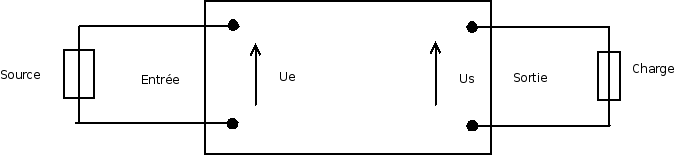
\includegraphics[width=12cm]{quadripole.png}
  \caption{Modèle du quadripôle}
\end{figure}
Si la source est une source de tension, on étudiera le cas où la source délivre un signal sinusoïdale ou échelon\\
Dans le cas sinusoïdale, on défini deux sous circuits : \\
\begin{figure}[ht]
  \centering
  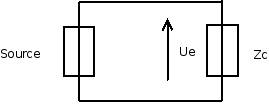
\includegraphics[width=5cm]{Physique/source.png}
  \caption{La source}
\end{figure}
\begin{figure}[ht]
  \centering
  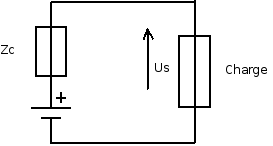
\includegraphics[width=6cm]{charge.png}
  \caption{La charge}
\end{figure}
\section{Fonction de transfert complexe}
\begin{de}
Dans le cas d'une sources fournissant un signal sinusoïdale, on défini une fonction de transfert par : 
$$H (j\omega) = \dfrac{\underline{X}_s}{\underline{X}_e}$$
avec :
\begin{itemize}
 \item[$\rightarrow$] $\underline{X}_s$ : Grandeur de sortie (Tension ou intensité)
 \item[$\rightarrow$] $\underline{X}_e$ : Grandeur d'entrée (Tension ou intensité)
\end{itemize}
Ces fonction de transfert sont sans dimensions.
\end{de}
\subsection{Amplitude}
Soit $\omega$ une pulsation, définie en rad.$s^{-1}$.\\
On associe à $\omega$ une fonction de transfert $H(j\omega)$.\\
\begin{de}
On appelle amplitude de H le module de H. 
$$(\mbox{ A est l'amplitude de H }) \Leftrightarrow ( A = |H(j\omega)|)$$
\end{de}
\subsection{Gain en décibel}
\begin{de}
On défini le gain en décibel d'une fonction de transfert par : 
$$G_{dB} = 20.log(|H(j\omega)|)$$
On utilise une échelle logarithmique pour pouvoir couvrir un large spectre de fréquence.
\end{de}
\subsection{Bande passante}
\begin{de}
On défini une bande passant comme l'ensemble des fréquences $\left\lbrace f \right\rbrace $ vérifiant :
$$| H(j2\pi f) | \geq \dfrac{H_{max}}{2} $$
\end{de}
\subsection{Phase}
\begin{de}
La phase de la fonction de transfert H($j\omega$) est l'argument de celui-ci.
\end{de}
\section{Représentations}
\subsection{Diagramme de Bode}
On défini deux graphiques : 
\begin{itemize}
 \item[$\rightarrow$] Celui du Gain : log(f) en abscisse, $G_{dB}$ en ordonnée
 \item[$\rightarrow$] Celui de la phase : log(f) en abscisse, $\varphi$ en ordonnée
\end{itemize}
\subsection{Diagramme de Nykwest}
On défini, dans le plan complexe, un point M qui à pour module $|H(j\omega)|$ et pour angle par rapport à l'axe de réel, $\varphi$
\section{Lien entre régime transitoire et fonction de transfert}
\subsection{Précaution d'utilisation}
Pour pouvoir utiliser ce procéder qui permet d'obtenir l'équation temporelle d'après la fonction de transfert, il faut que, lors de l'obtention de la fonction de transfert, si il existe plusieurs dipôles identiques dans le circuit, on les ai considérés de façon différente (ex : Si il y a deux résistance de valeur R, on pose qu'une est de valeur R, l'autre de valeur R', même si R=R').\\
A partir de là, on peut passer en temporel, et une fois l'équation différentielle obtenu, on utilise le faite que R=R'.
\subsection{Principe}
Considérons un quadripole. Pour déterminer l'équation différentielle relative au régime transitoire, on peut utiliser la fonction de transfert.\\
On considère donc que le circuit fonctionne en régime sinusoïdale. Une fois la fonction de transfert établie, on remplace les $(j\omega)^n\underbar{X}^n$ par $\dfrac{d^nX}{dt^n}$, et on obtient l'équation différentielle qui régit le système en régime transitoire.
\section{Type de réponse}
\subsection{Réponse indicielle}
La réponse indicielle est la réponse du système à un échelon.
\subsection{Réponse impulsionelle}
La réponse impulsionelle est la réponse du système à un échelon de longueur $\tau$.
\begin{prop}
Dans ce cas, on obtient la propriété suivante, qui est une propriété des transformée de Fourier : 
$$BP.\tau = 1$$
\end{prop}
\section{Réponse d'un filtre à un signal périodique}
Soit e(t) la tension d'entrée du quadripole.\\
Si e(t) est de la forme : 
$$e(t) = E.cos(\omega t)$$
Alors s(t), la tension de sortie du quadripole est donnée par :
$$s(t) = |H(j\omega)|.E.cos(\omega t + Arg(H(j\omega))$$
\section{Caractère intégrateur ou dérivateur d'un filtre}
\subsection{Filtre intégrateur}
\begin{de}
On dit d'un filtre qu'il est intégrateur si :
$$s(t) = \dfrac{1}{a}.\int e(t)$$
ou
$$e(t) = a.\dfrac{ds(t)}{dt}$$
Ce qui signifie que la fonction de transfert du système est de la forme (Intégrateur idéal) : 
$$H(j\omega) = \dfrac{1}{ja\omega}$$
\end{de}
\subsection{Filtre dérivateur}
\begin{de}
On dit d'un filtre qu'il est dérivateur si :
$$s(t) = b.\dfrac{de(t)}{dt}$$
Ce qui signifie que la fonction de transfert du système est de la forme (Dérivateur idéal) : 
$$H(j\omega) = jb\omega$$
\end{de}

 % Relue, correction orthographe
\chapter{Analyse d'un signal}
\section{Signal périodique}
Soit f une fonction.
\begin{de}
f est une fonction périodique si :
$$\exists T~ tq~ \forall t~ f(t+T) = f(t)$$
\end{de}
\subsection{Caractéristique principale}
Soit f une fonction périodique.
\subsubsection{Période, fréquence}
Ces deux caractéristiques sont fondamentale. La fréquence de la fonction est l'inverse de la période :
$$f = \dfrac{1}{T}$$
\subsubsection{Valeur moyenne}
\begin{de}
On défini la valeur moyenne d'une fonction f de la façon suivante : 
$$\left\langle f(t) \right\rangle = \dfrac{1}{T} \int_{t_0}^{t_0+T} f(t)dt $$
\end{de}
\subsubsection{Valeur efficace}
\begin{de}
On défini la valeur efficace d'une fonction f de la façon suivante :
$$F_e = \sqrt{\left\langle f^2(t) \right\rangle}$$
On peut l'écrire aussi sous la forme : 
$$F_e^2 = \dfrac{1}{T} \int_{t_0}^{t_0+T} f^2(t)dt$$
\end{de}
\section{Décomposition d'un signal périodique en fonction sinusoïdale}
\subsection{Théorème de Fourier}
\begin{enon}
Considérons une fonction périodique f : 
$$\exists T~ tq~ \forall t~ f(t+T) = f(t)$$
Il existe deux suites, ($a_n$) et $(b_n)$, telque : 
$$f(t) = \dfrac{a_0}{2} + \sum_{n=1}^{\infty} a_n\cos\left(\dfrac{2\pi n t}{T}\right) + \sum_{m=1}^{\infty} b_m\sin\left(\dfrac{2\pi m t}{T}\right)$$
\end{enon}
Les suites $(a_n)$ et $(b_n)$ sont appelé coefficients de Fourier.
\begin{enon}
$\forall n \in N$ : 
$$a_n = \dfrac{2}{T}\int_{t_0}^{t_0+T} f(t)\cos\left(\dfrac{2\pi nt}{T}\right)dt$$
$$b_n = \dfrac{2}{T}\int_{t_0}^{t_0+T} f(t)\sin\left(\dfrac{2\pi nt}{T}\right)dt$$
\end{enon}
\begin{prop}
On observe que : 
\begin{itemize}
 \item[$\rightarrow$] Si f est impaire, $\forall n \in N~ a_n=0$
 \item[$\rightarrow$] Si f est paire, $\forall n \in N~ b_n=0$
\end{itemize}
\end{prop}
\subsubsection{Coefficients de Fourier complexe}
\begin{prop}
En passant $\cos$ et $\sin$ en complexe, dans les coefficients de Fourier, on obtient que : 
$$f(t) = \sum_{-\infty}^{+\infty}c_n.e^{\frac{i2\pi nt}{T}}$$
avec : 
$$c_n = \dfrac{1}{T}\int_{t_0}^{t_0+T} f(t)e^{\frac{-i2\pi nt}{T}}dt$$
\end{prop}
\subsection{Identité de Parseval}
Soit f fonction périodique.\\
\begin{de}
Considérons le développement en série de Fourier de f : 
$$f(t) = \dfrac{a_0}{2} + \sum_{n=1}^{\infty} a_n\cos\left(\dfrac{2\pi n t}{T}\right) + \sum_{m=1}^{\infty} b_m\sin\left(\dfrac{2\pi m t}{T}\right)$$
On en déduit que : 
$$\left\langle f^2(t)\right\rangle = \dfrac{a_0}{4} + \sum_1^{\infty} \dfrac{a^2_n}{2} + \sum_1^{\infty} \dfrac{b²_n}{2}$$
car tous les doubles produits, issue de l'élévation au carré, qui comporte des fonctions cos ou sin ont une valeur moyenne nulle.
En posant :
$$c_n = \dfrac{a_n - ib_n}{2}$$
On obtient : 
$$\left\langle f^2(t)\right\rangle = \sum_{-\infty}^{+\infty} |c_n|^2$$
 
\end{de}

\subsection{Transformée de Fourier}
\begin{de}
Considérons f, une fonction.\\
On associe à f une fonction périodique $\overset{\sim}f$ : 
$$\forall t~ f(t) \rightarrow \overset{\sim}f(\nu)$$
Avec : 
$$\overset{\sim}f(\nu) = \int_{-\infty}^{+\infty} f(t)e^{-i2\pi\nu t}dt$$
On peut retourner cette égalité.
\end{de}

 % Relue, correction orthographe
\part{Electrostatique et Electrocinétique}
\setcounter{chapter}{0}
\chapter{Forme locale de l'électrostatique}
\section{Champs électrique}
\subsection{Définitions}
\begin{de}
Soit E une application :
$$E : M \mapsto \overrightarrow{E}(M)$$
Si en un point M, on place une charge $q_0$, cette charge subit une force $\overrightarrow{f}$.\\
On défini donc le champs électrique par : 
$$\overrightarrow{E} = \dfrac{\overrightarrow{f}}{q_0}$$
On observe donc que le champs électrique est indépendant de la charge $q_0$. On obtient donc qu'en introduisant un champs, on se libère du point d'observation.
\end{de}
\subsubsection{Loi de Coulomb}
\begin{de}
Soit A($q_1$) un point matériel de charge $q_1$, B($q_2$), un point matériel de charge $q_2$. La force exercé de A sur B est donnée par, avec $r = \parallel\overrightarrow{AB}\parallel$ : 
$$\overrightarrow{f} = \dfrac{q_1.q_2}{4\pi\varepsilon_0.r^2}.\dfrac{\overrightarrow{AB}}{AB}$$
Avec : 
$$\dfrac{1}{4\pi\varepsilon_0} = 9.10^9$$.
On en déduit : 
$$\overrightarrow{E}(M) = \dfrac{1}{4\pi\varepsilon_0.r^2}.\dfrac{q.\overrightarrow{AB}}{AB}$$
\end{de}
\subsubsection{Calcul direct du champs}
Considérons un volume chargée.\\
Considérons une charge élémentaire dans ce volume, notée dq : 
$$dq = \rho.dv$$
Avec $\rho$ la densité volumique de charge de ce volume, et $dv$ le volume élémentaire contenant cette charge dq.\\
Soit M un point de l'espace, et P un point appartenant à dq.
On obtient : 
$$\overrightarrow{E}(M) = \dfrac{1}{4\pi\varepsilon_0}\underset{source}\iiint \dfrac{\rho.\overrightarrow{PM}}{PM^3}.dv$$
\section{Potentiel électrique}
\begin{de}
En partant de l'expression de la force déterminer dans le paragraphe à propos de la loi de coulomb : 
$$\overrightarrow{f} = \dfrac{q_1.q_2}{4\pi\varepsilon_0.r^2}.\dfrac{\overrightarrow{OM}}{OM}$$
On obtient que, avec : 
$$\delta \omega = \overrightarrow{f}.\overrightarrow{dm}$$
$$\overrightarrow{OM} = r.\overrightarrow{u_r}$$
$$\overrightarrow{dm}=dr.\overrightarrow{u_r}+r.d\theta.\overrightarrow{u_{\theta}}+r.sin(\theta)d\varphi.\overrightarrow{u_{\varphi}}$$
Donc : 
$$\delta \omega = -\dfrac{d}{dr}(\dfrac{q.q'.r}{4\pi\varepsilon_0})$$
On peut donc introduire une énergie potentielle (au sens mécanique du terme).
$$E_p = q'.\dfrac{q}{4.\pi.\varepsilon_0.r} = q'.V(m)$$
D'ou :
$$\overrightarrow{E}(M).\overrightarrow{dm} = -dV$$
On peut écrire cette relation sous la forme : 
$$\overrightarrow{E}(M) = -\overrightarrow{grad}V$$
En partant de l'expression du grandiant de V et de l'expression $\overrightarrow{dm}$ dans un système de coordonnée, on peut déterminer l'expression du champs électrique.
\end{de}
\subsection{Calcul direct du potentiel}
\begin{de}
Considérons un volume chargé, de densité volumique de charge $\rho$.\\
Considérons un volume élémentaire dv, avec P appartenant à dv, et M un point de l'espace :
$$V(M) = \underset{V charge}\iiint \dfrac{\rho.dv}{4\pi\varepsilon_0.PM}$$
\end{de}
\subsection{Condition pour qu'un champs de vecteurs soit un gradiant}
Soit $\overrightarrow{D}(M)$ un champs de vecteur.\\
Soit $\overrightarrow{rot}(\overrightarrow{D})$, le rotationnel de D, défini par : 
$$\overrightarrow{rot}\overrightarrow{D} = (\dfrac{\partial D_z}{\partial y}-\dfrac{\partial D_y}{\partial z};\dfrac{\partial D_x}{\partial z}-\dfrac{\partial D_z}{\partial x};\dfrac{\partial D_y}{\partial x}-\dfrac{\partial D_x}{\partial y})$$
Si $\overrightarrow{rot}(\overrightarrow{D}) = \overrightarrow{0}$, alors :
$$\exists g~ tq~ \overrightarrow{D}(M) = \overrightarrow{grad}(f)$$
\subsection{Lien entre direction de champs et surface equipotentielle}
\begin{prop}
$\overrightarrow{E}(M)$ sera parralèle à la surface équipotentielle V(M), avec $\overrightarrow{E}(M)$ dirige vers les potentiels décroissants
\end{prop}
\section{Théorème de Gauss}
\begin{enon}
Le flux du champ électrique à travers une surface fermé $\Sigma$ orienté vers l'extérieur est égale à la charge intérieur à cette surface sur la permitivité du vide, $\varepsilon_0$ : 
$$\phi = \underset{\Sigma}\oiint \overrightarrow{E}.\overrightarrow{n}.dS = \dfrac{Q_{int}}{\varepsilon_0}$$
\end{enon}
\begin{prop}
D'après le théorème de Gauss, on peut déduire que le potentiel ne peut pas être extremum au niveau d'un point vide de charge.
\end{prop}
\subsection{Forme locale du théorème de Gauss}
\subsubsection{Opérateur Divergence}
\begin{de}
On défini l'opérateur divergence, notée div, par : 
$$div : \Re^3 \rightarrow \Re$$
$$\overrightarrow{D} \mapsto div(\overrightarrow{D})$$
Supposons que $\overrightarrow{D}(x,y,z)$, alors :
$$div(\overrightarrow{D}) = \dfrac{\partial D_x}{\partial x} + \dfrac{\partial D_y}{\partial y} + \dfrac{\partial D_z}{\partial z}$$
\end{de}
\begin{prop}
Considérons une surface fermé $\Sigma$, de volume intérieur chargé V : 
$$\phi = \underset{\Sigma}\iint\overrightarrow{E}(M).\overrightarrow{n}.dS = \underset{V}\iiint div(\overrightarrow{E}).dV$$
\end{prop}
\subsection{Équation de Poisson}
\subsubsection{Opérateur Laplacien}
\begin{de}
On défini l'opérateur Laplacien, noté $\Delta$, par : 
$$\Delta : \Re \rightarrow \Re$$
$$A \mapsto \Delta(A)$$
Avec : 
$$\Delta(A) = \dfrac{\partial^2 A}{\partial^2 x} + \dfrac{\partial^2 A}{\partial^2 y} + \dfrac{\partial^2 A}{\partial^2 z}$$ 
\end{de}
\subsubsection{Énoncé}
Considérons une surface fermé, $\Sigma$, de densité volumique de charge $\rho$, de volume chargé V.\\
D'après le théorème de Gauss, on obtient que : 
$$\phi = \underset{\Sigma}\oiint\overrightarrow{E}(M).\overrightarrow{n}.dS = \underset{V}\iiint \dfrac{\rho.dV}{\varepsilon_0} = \underset{V}\iiint div(\overrightarrow{E}).dV$$
On en déduit donc le relation locale suivante, qui dépend du point M :
$$\dfrac{\rho}{\varepsilon_0} = div(\overrightarrow{E})$$
Or, par définition : 
$$\overrightarrow{E} = -\overrightarrow{grad}(V)$$
On obtient donc que : 
$$div(\overrightarrow{E}) = -\Delta(V)$$
Avec $\Delta(V)$ le Laplacien de V.\\
On obtient donc que : 
$$\dfrac{\rho}{\varepsilon_0} = -\Delta V$$
Ceci constitue l'équation de poisson.
 % Relue, correction orthographe
\chapter{Conducteur électrique en équilibre}
\section{Définitions}
\subsection{Conducteur}
\begin{de}
Un conducteur est un composant qui contient des charge mobiles, susceptible de ce déplacer.
\end{de}
\begin{de}
On dit qu'un conducteur est à l'équilibre si il est à l'équilibre mécanique.\\
Toutes les charges à l'intérieur de ce conducteur doivent être à l'équilibre mécanique.\\
Considérons une charge mobile. Cette charge est à l'équilibre si :
$$\sum \overrightarrow{F} = \overrightarrow{0}$$
\end{de}
\section{Propriétés de l'équilibre pour un conducteur donnée}
\subsection{Conséquence des définitions globale}
\subsubsection{Le champs électrique est nul à l'intérieur d'un conducteur}
Considérons un électron.\\
Le système est à l'équilibre, on obtient donc : 
$$q.\overrightarrow{E}+m.\overrightarrow{g} = \overrightarrow{0}$$
Ce qui implique que : 
$$\overrightarrow{E} = \dfrac{-m.\overrightarrow{g}}{q}$$
Par application numérique, on obtient un champs électrique de l'ordre du $10^{-11}$.\\
On peut donc considérer qu'à l'équilibre, sont champs équilibre est nul.
\subsubsection{Le conducteur est un volume équipotentiel}
Sachant que :
$$\overrightarrow{E} = -\overrightarrow{grad}(V)$$
On obtient, qu'a l'équilibre, comme le champs est nul, le potentiel est une constante.\\
Un conducteur à l'équilibre est donc un volume équipotentiel
\subsubsection{La densité volumique de charge est nul dans un conducteur}
Nous avons vu que : 
$$div(\overrightarrow{E}) = \dfrac{\rho}{\varepsilon_0}$$
Ceci implique que $\rho=0$. À l'intérieur du conducteur, les charges se compensent. L'excédent de charge est porté par la surface. Il y a donc une densité surfacique de charge.
\subsection{Cavité vide de charge dans un conducteur}
En considérant le faite qu'on ne peut pas avoir un extremum du potentiel dans une zone vide de charge, et qu'il y à continuité du potentiel à la traversé de la surface, le potentiel dans la cavité est le même que dans le conducteur.
\subsection{Champs électrique à la surface du conducteur}
Nous avons vu : 
$$\overrightarrow{E}_{int}-\overrightarrow{E}_{ext} = \dfrac{\sigma}{\varepsilon_0}\overrightarrow{n}$$
Or le champs intérieur est nul dans un conducteur à l'équilibre, nous l'avons vu. On obtient donc que : 
$$E_{ext} = \dfrac{\sigma}{\varepsilon_0}$$
La mesure du champs électrique extérieur permet donc de connaître la densité surfacique $\sigma$.
\section{Système de conducteur en équilibre}
\subsection{Il y a unicité des solutions}
Considérons un ensemble de conducteurs. On démontre que si on à un ensemble de conducteur, et si on fixe des conditions (ex : La charge $q_i$ ou le potentiel $V_i$ du conducteur i), alors $V(M)$ est fixé (Et non défini à une constante près, comme habituellement).\\
De plus, on as : 
$$\Delta V = \dfrac{\rho}{\varepsilon_0} = 0$$
Car l'espace entre les conducteurs est vide de charge. On fait appelle aux conditions appelé conditions limite : 
\begin{itemize}
 \item[$\rightarrow$] Si $V_i$ est connu, à l'aide d'une relation de continuité par exemple
 \item[$\rightarrow$] Si $q_k$ est connu, à l'aide d'une surface de Gauss par exemple
\end{itemize}
Alors il existe une solution unique pour définir V(M)
\subsection{Conducteur seul dans l'espace}
On pose la relation suivante : 
$$Q = C.V$$
Avec Q la charge, C la capacité du conducteur, et V le potentiel.\\
Considérons une sphère de rayon r.\\
On obtient à l'aide d'une surface de Gauss que : 
$$V = \dfrac{Q}{4\pi\varepsilon_0.r}$$
En posant que le potentiel est nul à l'infini (pour la constante).\\
On obtient donc quand ce cas que : 
$$C = 4\pi\varepsilon_0$$
\subsection{Influence électrique}
Considérons une sphère métallique conducteurs.\\
Si on rapproche une charge de ce conducteur, la répartition des charges en surface est modifié, mais $\rho$, la densité volumique de charge demeure nulle.
\section{Condensateur}
\begin{de}
Un condensateur est composé de deux conducteur en influence totale.
\end{de}
\subsection{Capacité d'un condensateur}
Considérons un condensateur composée de deux conducteur sphérique 1, de charge $Q_1$ et 2, de charge intérieur (surface la plus proche de 1) $Q_{2~ int}$, et de charge extérieur $Q_{2~ ext}$, avec 1 intérieur à 2.\\
Considérons une surface $\Sigma$ sphérique contenu dans 2. Les conducteurs étant à l'équilibre, on obtient que : 
$$\forall M \in \Sigma~ \underset{\Sigma}\iint \overrightarrow{E}(M).\overrightarrow{n}.dS = 0 = \dfrac{Q_1 + Q_{2~ int}}{\varepsilon_0}$$
Ceci implique que : 
$$Q_{2~ int} = -Q_1$$
Considérant maintenant un point M extérieur à 2. On obtient : 
$$\iint \overrightarrow{E}(M).\overrightarrow{n}.dS = \dfrac{Q_1 + Q_{2~ int}+ Q_{2~ ext}}{\varepsilon_0} = \dfrac{Q_{2~ ext}}{\varepsilon_0}$$
Le champs entre les armatures ne dépend que de $Q_1$. On obtient donc :
$$Q_1 = C.(V_1-V_2)$$
 % Relue, correction orthographe
\chapter{Complément d'électrocinétique}
\section{Définitions}
\subsection{Intensité de courant}
\begin{de}
L'intensité est un débit de charge : 
$$i = \dfrac{dq}{dt}$$
\end{de}
\subsection{Vecteur densité surfacique de courant}
\begin{de}
On considère une surface $\Sigma$. On peut écrire : 
$$ i = \underset{\Sigma}\iint \overrightarrow{j}.\overrightarrow{n}.dS$$
Avec $\overrightarrow{j}$ le vecteur densité surfacique de courant.
\end{de}
Considérons un modèle composé d'un seul type de porteur de charge. \\
On obtient que : 
$$dq = \rho_m.\overrightarrow{v}.\overrightarrow{n}.\Sigma.dt$$
On peut identifier et on obtient que :
$$\overrightarrow{j} = \rho_m.\overrightarrow{v}$$
Avec $\rho_m$ la densité de charge mobile. Par un théorème de superposition, on obtient dans un modèle de multiple porteur de charge : 
$$\overrightarrow{j} = \sum \rho_{m,i}.\overrightarrow{v_i}$$
\subsection{Équation de continuité}
Considérons un conducteur fermé de surface $\Sigma$. Nous avons les équations suivantes :
$$i = \underset{\Sigma}\iint \overrightarrow{j}.\overrightarrow{n}.dS$$
$$i = \dfrac{-dQ}{dt}$$
$$Q = \iiint_v \rho.dv$$
En considérant que cette surface est invariente avec le temps, on obtient que : 
$$\dfrac{\partial \rho}{\partial t} + div(\overrightarrow{j}) = 0$$
Ceci est une équation locale, car toute ces composantes dépendent du point M. Cette équation est l'expression de la conservation de la charge.\\
On en déduit qu'en régime permenant, conscient que dans ce cas $\rho$ est une constante par rapport au temps : 
$$div(\overrightarrow{j})= 0$$
\section{Expression de la puissance reçu par un dipôle}
Considérons un dipôle contenant des charges mobiles. En discrétisant le problème, on obtient l'expression du travail :
$$\omega = \sum q_i.\overrightarrow{E}(m_i).\overrightarrow{v_i}.dt$$
Cette somme est a réaliser sur l'ensemble des charges mobiles. Dans le cas continue, on obtient : 
$$\omega = \underset{v}\iiint \rho_{mobile}.d\tau.\overrightarrow{E}(M)<\overrightarrow{v}>dt$$
D'ou l'expression de la puissance, sachant que : 
$$P = \dfrac{d\omega}{dt} = \underset{v}\iiint \rho_{mobile}.d\tau.\overrightarrow{E}(M)<\overrightarrow{v}>$$
D'ou : 
$$P = \underset{v}\iiint \overrightarrow{j}.\overrightarrow{E}(M).d\tau$$
Cette expression est l'expression de la puissance reçu par le dipôle.\\
Au finale, on obtient donc que : 
$$P=i*(V_A-V_B)$$
Avec A et B respectivement le point d'entre et le point de sortie du dipôle.
\section{Conducteur ohmique}
\subsection{Loi d'Ohm}
Soit la loi d'Ohm : 
$$U = R.i$$
Cette relation revient à dire que : 
$$\overrightarrow{j} = \sigma.\overrightarrow{E}$$
Avec $\sigma$ la conductivité.\\
La loi d'ohm ne s'applique que si $\rho_m$ est une constante indépendante de $\overrightarrow{E}$. En pratique, un dipôle vérifie la loi d'ohm dans un certain intervalle de valeur pour $\overrightarrow{E}$.
\subsection{Résistance électrique}
\begin{de}
Considérons un dipôle électrique. On suppose qu'il vérifie la loi d'ohm, donc : 
$$\overrightarrow{j}=\sigma.\overrightarrow{E}$$
De plus, nous avons les équations suivantes :
$$i = \underset{\Sigma}\iint \overrightarrow{j}.\overrightarrow{n}.dS$$
$$\overrightarrow{E} = -\overrightarrow{grad}(V)$$
On en déduit donc que : 
$$V_A - V_B = \int_A^B \overrightarrow{E}.\overrightarrow{dm}$$
On obtient donc que :
$$V_A - V_B = R.i$$
Avec R une constante, appelé résistance
\end{de}
\begin{prop}
On remarque des corrélations entre la capacité et la résistance d'un dipôle. On montre que dans une topologie proche, on as : 
$$R.C = \dfrac{\varepsilon_0}{\sigma}$$
\end{prop}
\subsection{Effet Joule}
Considérons un dipôle. Soit P la puissance reçu par ce dipôle. On obtient : 
$$P = \iiint \overrightarrow{j}.\overrightarrow{E}.d\tau$$
Or dans le cas d'un conducteur ohmique : 
$$\overrightarrow{j} = \sigma \overrightarrow{E}$$
Donc : 
$$P = \iiint \sigma.E^2.d\tau > 0$$
Donc un conducteur ohmique ne peut que consommé de l'énergie.
  % Relue, correction orthographe
\part{Thermodynamique}
\setcounter{chapter}{0}
\chapter{Rappel et complément - Thermodynamique classique}
\section{Principe}
\subsection{Principe zéro}
\begin{enon}
Si on prend un système isolé, celui-ci évolue vers un état d'équilibre
\end{enon}
Ce principe est celui de l'existence d'état d'équilibre.\\
Dans ces états d'équilibre, les grandeurs thermodynamique, grandeurs macroscopique, sont parfaitement définies.
\subsubsection{Grandeur intensive, extensive}
\begin{de}
Une grandeur est extensive si l'addition a un sens pour elle. Si ça n'est pas le cas, la grandeur est dit intensive
\end{de}
\subsection{Premier Principe}
\begin{enon}
Le premier principe est un principe d'évolution
Il existe une grandeur, appellé énergie totale, extensive et conservative, que l'on peut définir dans tous système fermé.
On appelle énergie totale d'un système, toutes l'énergie présente, peu importe sa forme.
$$E_{tot}=E_{m,M}+u+E_{nucl}+E_{autre}$$
L'énergie est une fonction d'état. Elle ne dépend pas du chemin suivit, mais uniquement de l'état de départ et de l'état d'arrivé.\\
La varitation de cette énergie est donnée par : 
$$\Delta E = w + Q$$
\end{enon}
\subsubsection{Enthalpie}
\begin{de}
Soit enthalpie, fonction d'état notée H, la fonction définie par : 
$$H = u+pV$$
Avec u énergie interne, p la pression et V le volume. 
\end{de}
\begin{prop}
Dans le cas d'une transformation monobar (pression exterieur constante), on as :
$$Q = \Delta H$$
\end{prop}
\subsubsection{Extension du premier principe à un systeme ouvert}
\begin{prop}
On peut etendre ce principe à u système ouvert. Par exemple, dans le cas d'une fluide en écoulement, on prend comme système : Systeme ouvert (Machine) + fluide qui entre pour l'instant t, et Systeme ouvert (Machine) + fluide qui sorte à l'instant t+dt.\\
Dans ce cas, on peut appliquer le premier principe à ce système.
\end{prop}

\subsection{Second principe}
\begin{enon}
Énoncé de Thompson :\\ 
Une machine ne peut pas effectuer un travail si elle n'est en contact qu'avec une seul source de chaleur
\end{enon}
\begin{enon}
Énoncé de Clausius :\\
Il ne peut pas y avoir de transformation donc le seul effet serai de transporter de la chaleur d'une source froide vers une source chaude.
\end{enon}
\subsubsection{Entropie}
\begin{enon}
Pour tous système fermé, on peut définir une fonction d'état, notée S, appelé entropie, qui serai une grandeur extensive, mais non conservative. Cette grandeur peut être crée ou non, mais jamais détruite.
\end{enon}
\begin{de}
Le bilan entropique est défini par :
$$\Delta S = S^{r}+S^{p}=\int dS$$
$$S^{r}=\int \dfrac{\delta Q}{Tf}$$
Si le système est caractérisé par T,V, on a :
$$dS = \dfrac{du}{T}+\dfrac{p.dV}{T}$$
Si il est caractérisé par p,T, on a :
$$dS = \dfrac{dH}{T}-\dfrac{V.dp}{T}$$
On détermine $S^{p}$ à l'aide de la relation :
$$S^{p} = \Delta S - S^{r}$$
\end{de}
\subsubsection{Température}
À l'aide de l'expression de dS dans le cas d'un système caractérisé par T,V, on peut définir la température par : 
$$\dfrac{1}{T} = \left(\dfrac{\partial S}{\partial u}\right)_V$$
\section{Quelques notions de mécanique statique}
\subsection{Modèle cinétique du gaz parfait}
\begin{de}
On montre que la pression exercé par N molécule de masse m, dans un volume V est donnée par : 
$$P = \dfrac{N.m.<v^2>}{V.3}$$
Avec $<v^2>$ la vitesse quadratique moyenne des molécules.
\end{de}
\begin{de}
On défini la constant de Boltzman, notée k, par : 
$$k = \dfrac{R}{Na}$$
Avec R la constante des gaz parfait, et Na le nombre d'Avogadro.
\end{de}
\begin{de}
Chaque terme énergétique ajoute un terme en $\dfrac{1}{2}R$ dans la capacité calorifique à volume constant dans le modèle des gaz parfait.\\
Pour un gaz parfait diatomique, on défini : 
\begin{enumerate}
 \item[$\rightarrow$] $C_v = \dfrac{3}{2}R$ a basse température ( Translation )
 \item[$\rightarrow$] $C_v = \dfrac{5}{2}R$ a température ambiante ( Translation + rotation )
 \item[$\rightarrow$] $C_v = \dfrac{7}{2}R$ a haute température ( Translation + rotation + vibration )
\end{enumerate}
\end{de}

\subsection{Interprétation statistique de l'entropie}
\begin{de}
Un état macroscopique est constitué de multiples états microscopique. Boltzman défini l'entropie par :
$$S = k.ln(\Omega)$$
Avec $\Omega$ le nombres d'états microscopique constituant l'état macroscopique.\\
L'entropie augmente donc quand le nombres d'état microscopique augmente. 
\end{de}
\section{Gaz parfait}
\subsection{Équation d'état des gaz parfaits}
\begin{de}
L'équation d'état des gaz parfaits est : 
$$p.V = n.R.T$$
Avec p, la pression exprimé en Pa ( 1 bar = $10^5$ Pa), le volume en $m^3$, n en moles et T en Kelvin.\\
R, la constante des gaz parfait, est donnée par :
$$R = 8,314~ J.K^{-1}.mol^{-1}$$
Cette équation est du à Gay-Lussac.
\end{de}
\begin{de}
Cette équation est éloigné des résultats expérimentaux. On utilise un "variante" de cette équation, appellé equation de Van der Walles. Cette équation est : 
$$\left( p + \dfrac{a}{V^2}\right).(V-b) = R.T$$
Dans cette équation, on prend en compte le covolume (le volume des atomes), ce qui réduit le volume disponible, et on considère les interactions entre atomes, ce qui diminue la pression. Ces deux choses ne sont pas considéré dans le modèle du gaz parfait.
\end{de}
\subsection{Loi de Joules}
\subsubsection{Premier loi de Joules}
\begin{enon}
Le première loi de Joules postule que u est une fonction qui dépend uniquement de la température. u=f(T)
\end{enon}
\begin{prop}
À partir de cette loi, on peut voir que : 
$$du = \dfrac{\partial f}{\partial T}dT = n.C_v.dT$$
\end{prop}
\subsubsection{Deuxième loi de Joules}
\begin{enon}
La deuxieme loi de Joules dit que, a l'aide de l'équation d'état des gaz parfaits : 
$$H = U + pV = f(T) + n.R.T = F(T)$$
Donc l'enthalpie est aussi une fonction de la température. De plus :
$$dH = n.C_p.dT \Rightarrow C_p = G(T)$$
La capacité calorifique à pression constante est donc aussi une fonction de la température.\\
D'après ces expression, on en déduit que : 
$$n.C_p = n.C_v + n.R$$
On obtient donc la relation de Mayer :
$$C_p - C_v = R$$
\end{enon}
\subsection{Entropie}
\begin{de}
On appelle identité thermodynamique la relation suivante :
$$du = \delta Q + \delta w$$
\end{de}
\begin{prop}
D'après l'identité thermodynamique, et sachant que : 
$$dH = du + d(pV)$$
On obtient : 
$$dH = \delta Q + \delta w + pdV+Vdp$$
Sachant que H et u sont des fonctions d'état, donc ne dépendent pas du chemin suivit, mais uniquement de l'état de départ et de l'état d'arrivé, on peux considérer un transformation réversible. On obtient donc :
$$\delta Q_{rev} = T_fdS$$
Donc :
$$dH = T_fds + Vdp$$
En développement à l'aide de l'entropie, dans le cas d'une transformation adiabatique quasi statique d'un gaz parfait,  on obtient la relation de Laplace : 
$$p.V^{\gamma} = cte$$
Avec $\gamma$ défini par : 
$$\gamma = \dfrac{C_p}{C_v}$$
\end{prop}

\chapter{Potentiel Chimique}
\section{Enthalpie libre}
\subsection{Travail récupérable dans une transformation monotherme, monobar}
Considérons une transformation monotherme, le système est en contact avec un thermostat, et monobar, la pression exterieur au système est constante ( Ce genre de transformation est le cas global en chimie).\\
Par application du premièr principe : 
$$\Delta u = w + Q$$
D'ou, avec $w_a$ un travail autre que les forces de pression :
$$w_a = \Delta u + p_0\Delta V - T_0 \Delta S - T_0 \Delta S^p = \Delta G^* + T_0 \Delta S^p$$
Donc $-w_a$, le travail récupérable, est limité par : 
$$w_a \leq \Delta G^*$$
\subsection{Enthalpie libre}
On introduit G, une fonction d'état, appelé enthalpie libre, qui est la fonction d'état le plus approprié pour étudier un systeme chimique subissent une évolution monobar et monotherme. On peut en effet exprimé H en fonction de G, nous le verrons.\\
Posons : 
$$G = U + pV - TS = H - TS$$
D'où :
$$dG = \delta w_a + Vdp - SdT - TdS^p$$
Dans ce cas, si $w_a = 0$: 
$$\Delta G \leq 0$$
G ne peut que diminuer au cours de l'évolution. L'état d'équilibre est atteint pour le minimum de cette fonction.
\subsection{Relation de Gibbs-Helmotz}
Considérons un système réversible soumis uniquement à des forces de pression.\\
Dans ce cas :
$$dG = VdP - SdT$$
D'ou : 
$$S = -\dfrac{\partial G}{\partial T}$$
En utilisant la deuxième définition de G donné dans l'étude de l'enthalpie libre, on obtient que : 
$$H = G - T\left( \dfrac{\partial G}{\partial T}\right)_{p,etc..} $$
D'ou : 
$$\dfrac{H}{T^2} = -\dfrac{\partial}{\partial T } \left(\dfrac{G}{T} \right) $$
\section{Potentiel chimique}
\begin{de}
Considérons un système chimique, par exemple $C + O_2 \rightarrow CO_2$. Ce système est caractérisé par T,P,V,$n_i$, avec $n_i$ les quantites de matière des entités présente.\\
L'enthalpie libre est donc une fonction de ces variables. Soit $\mu_i$, le potentiel chimique de l'entité i, défini par : 
$$\mu_i = \left( \dfrac{\partial G}{\partial n_i}\right)_{T,P,n_j} $$
\end{de}
\subsection{Relation d'Euler}
\begin{enon}
Soit $n_i$ la quantité de matière de l'entité i, et $\mu_i$ sont potentiel chimique. Notons l'une des entités chimiques $i0$.\\
On obtient la relation d'Euler, en considérant un système "séparer vituellement" en deux partie, avec une partie négligable devant l'autre :
$$G(T,P) = \sum_i \mu_i.n_{i}$$
\end{enon}
\subsection{Relation de Gibbs-Duhem}
\begin{enon}
D'après la relation d'Euler, on obtient que : 
$$Vdp - SdT = \sum_i n_i.d\mu_i$$
\end{enon}
\subsection{Équilibre d'un corps présent sous deux phases}
Considérons un système contenant deux solvants, Eau et Huile par exemple, et un corps présent dans chaqu'un de ces deux solvants\\
On défini l'enthalpie libre de ce systeme comme la somme de l'enthalpie libre des deux sous systèmes.\\
On obtient que le corps va migrer dans la phase où le potentiel chimique est le plus faible. Or nous avons vu que :
$$\mu_i(T,P,n_i)$$
Donc le potentiel chimique va varie avec $n_i$. L'équilibre du système est donc atteint quand la variation d'entalpie libre du système est nul, donc quand les potentiels chimiques seront égaux.
\section{Expression du potentiel chimique}
\subsection{Gaz parfait pur}
On obtient la relation suivante : 
$$\mu(T,P) = \mu(T,P_0) + R.T.ln\left(\dfrac{P}{P_0}\right)$$
Avec $P_0$ une pression de référence, qui est de 1 bar par convention.
\subsection{Gaz réel pur}
Dans le cas d'un gaz réel pur, on utilise un développent de Viriel, qui remplace d'équation d'équation d'états des gaz parfait par : 
$$\dfrac{p.V}{R.T}= n (1+\dfrac{A(T)}{V}+\dfrac{B(T)}{V^2} +\dfrac{C(T)}{V^3} + \dots)$$
On obtient donc, la relation suivante :
$$\mu(T,P) = \mu(T,P_0) + R.T.ln\left(\dfrac{f}{P_0}\right)$$
Avec f la fugacité du gaz, qui dépend des coefficiants A(T), B(T), C(T), $\dots$.
\subsection{Gaz parfait dans un mélange de gaz parfait}
Considérons un mélange constitué de deux gaz parfait.\\
On obtient la relation suivante : 
$$\mu_{i_{melange}}(T,P) = \mu_{i_{pur}}(T,P_0) + R.T.ln\left(\dfrac{P_i}{P_0}\right)$$
Avec $P_i$, la pression partiel de l'entité i, c'est à dire la pression qu'exercerai le gaz si il était seul dans le système.
\subsection{Phase condensée pur}
Dans l'étude des phases condensée, on arrive à la conclusion que : 
$$\mu(T,P)\simeq\mu(T,P_0)$$
Le potentiel chimique ne dépend plus que de la température
\subsection{Mélange idéale - Mélange homogène}
\begin{de}
On défini un mélange homogène comme un mélange dont la composition est identique en tout point.
\end{de}
Considérons un mélange composé de $n_e$ mole d'eau, et de $n_a$ molécule d'alcool. Il y a une phase liquide et une phase gazeuse. À l'équilibre, il y a égalité des potentiels chimiques.\\
On obtient : 
$$\mu_{A_{solution}} = \mu_{A_{pur}}(T,P) + R.T.ln\left(\dfrac{P_a}{P_{sa}}\right)$$
Avec $P_i$ la pression partiel de l'entité A, et $P_{sa}$ la pression de vapeur saturante de l'entité A.
\subsection{Solution diluée}
Considérons deux composants, A, le solvant, B, le soluté, avec $n_b \ll n_a$\\
On obtient : 
$$\mu_{B_{solution}}(T,P,compo) = f(T,P) + R.T.ln(x_b)$$
On peut obtenir cette relation à l'aide de la relation de Gibbs-Duhelm
\begin{enon}
On a donc :
$$Vdp -SdT = \sum_i n_i.d\mu_i$$
Si P est constant, tout comme T, on obtient donc :
$$\sum_i n_i.d\mu_i = 0$$
Donc 
$$-n_a.\dfrac{\partial \mu_a}{\partial x_b} = n_b \dfrac{\partial \mu_b}{\partial x_b}$$
Grace à ceci on obtient la relation ci dessus.
\end{enon}
Cette relation est vérifié dans le cas d'une solution infiniment dilué. Si la solution n'est que dilué, on fait appelle à l'activité.
$$\mu_{B_{solution}}(T,P,compo) = f(T,P) + R.T.ln(a_b)$$
Avec $a_b$ l'activité de l'espèce b.

\chapter{Équilibre liquide-vapeur d'un mélange binaire}
\section{Équilibre liquide-vapeur pour un corps pur}
\subsection{Équilibre d'un corps pur sous deux phases}
Considérons un corps pur présent sous deux phases, liquide et gazeux.\\
Si on considère une transformation monotherme et monobar, on obtient que :
$$\Delta G \leq 0$$
On en déduit que le système évolue toujours vers la phase avec le potentiel chimique le plus faible.\\
À l'équilibre chimique, on à :
$$\mu_l(T,P) = \mu_v(T,P)$$
La pression d'équilibre est donc une fonction de la température.\\
De cette considération, on obtient les diagrammes visible dans les fiches de révision de Sup, dans les changements d'états.
\subsection{Chaleur latente de changement d'état}
\begin{de}
On considère un système de 1 kilogramme. A pression constant, on obtient un palier à température constante, dans le diagramme T = f(t)\\
Un corps pur est défini comme un corps admettent un palier de changement d'état.
\end{de}
\begin{de}
La chaleur latente est l'énergie à fournir à 1 kilogramme de matière pour effectuer le changement d'état.\\
On obtient :
$$L = \Delta H_{vaporisation}$$
L'enthalpie etant une fonction d'état, on peut imaginer une transformation réversible pour effectuer le changement d'état. On obtient donc que : 
$$\Delta S = \dfrac{\Delta H}{T_v}$$
\end{de}
\subsection{Relation de Clapeyron}
Supposons que le système soit à l'équilibre à la température $T_1$ et à la pression $P_1$.\\
On as donc : 
$$\mu_l(T_1,P_1) = \mu_v(T_1,P_1)$$
On peut considérer qu'à la température $T_1 + dT$ et à la pression $P + dP$, le système est encore à l'équilibre.
On en déduit que :
$$\Delta  \mu_l = v_ldP - s_ldT$$
avec $v_l$ et $s_l$ des grandeurs molaires. Sachant qu'on obtient la même relation pour $\Delta \mu_v$, on obtient que : 
$$L = \dfrac{T_v(v_v-v_l)dP}{dT}$$
Ceci constitue la relation de Clapeyron. On peut d'après cette relation, en considérent le signe de L, déterminer la pente de la courbe de changement d'état dans un diagramme p = f(T), sachant que L est positif lors du changement d'état d'un état ordonnée vers un état moins ordonné.
\section{Équilibre liquide-vapeur d'un mélange binaire}
\begin{de}
On défini un mélange binaire comme un mélange composée de deux entités, qui peuvent être en phase liquide ou en phase gazeuse (ou inclusif ..)
\end{de}
Considérons un système composé de deux entités, a et b, avec $n_a$ et $n_b$ les quantités de matière de a et b en phase liquide, $n_a'$ et $n_b'$ les quantités de matière de a et b en phases gazeuse.\\
Dans l'étude d'un tel système, on défini les factions molaires suivante : 
$$x_a = \dfrac{n_a}{n_a + n_b}~ et~ x_b = 1 -x_a$$
$$x_a' = \dfrac{n_a}{n_a' + n_b'}~ et~ x_b' = 1 -x_a'$$
Le système est caractérisé par :
$$T,P,x_a',x_a$$
Or, à l'aide de la relation qui dit que les potentiels chimiques des phases gazeuse et liquide sont égaux à l'équilibre, on obtient deux équations liant ces quatres inconnues.\\
Le système est donc divariant, il ne dépent que de deux inconnues.
\section{Mélange de deux constituants totalements miscible à l'état liquide}
\subsection{Mélange idéale}
Considérons deux constituants, a et b.\\
Nous avons les hypothèses suivantes : 
$$P_a = x_a.P_{sa}(T)$$
$$P_b = x_b.P_{sb}(T) = (1-x_a)P_{sb}(T)$$
On obtient donc que : 
$$P = P_a+P_b = P_{sb}(T) + x_a(P_{sa}(T)-P_{sb}(T))$$
\subsubsection{Diagramme isotherme}
On en déduit que dans un diagramme isotherme, la pression est une fonction affine du titre $x_a$, le titre du liquide.\\
Si on considère le titre en vapeur, $x'_a$, on obtient que : 
$$P = \dfrac{P_{sb}}{1-x'a(1-\dfrac{P_{sb}}{P_{sa}})}$$
On obtient donc une hyperbole.\\
Soit $x''_a$ le nombre de mole de a (liquide + vapeur), sur le nombre totale de moles du système. Pour qu'il y ai équilibre liquide vapeur, il faut que ce titre soit compris entre les deux courbes.
\subsubsection{Diagramme isobare}
Les relations démontrer précédement reste valable. On obtient, en fixant la pression un diagramme isobare
\subsubsection{Règle des segments inverse}
Soit y, la grandeur défini par : 
$$y = \dfrac{x''_a-x'_a}{x_a-x_a'}$$
On obtient que : 
$$y=\dfrac{d(MV)}{d(LV)}$$
avec d(XZ) la distance entre X et Z.
\subsection{Mélange réel}
On peut toujours construire les diagrammes à l'aide d'expérience. On observe par contre des diagrammes avec un ou deux fusceaux, et des points azéotropique.
\subsubsection{Points azéotropique}
Un point azéotropique est un point de rencontre des deux courbe f($x_a$) et $f(x'_a)$, par exemple.\\
En ce point, le changement d'état s'effectue a temperature constante. On pourrai donc croire que le mélange binaire est un corps pur, car l'existance de ce palier est l'une de leurs caractéristique. Mais ce point azéotropique dépend de la pression, donc le palier dépend de la pression à la quelle on travaille, ce qui n'est pas le cas pour un corps pur.\\
Ces point ont une forte influence, dans la distilation par exemple, car on ne peut pas dissocier les deux composants. On peut dissocier un composant et un mélange azéotrope.

\chapter{Grandeurs thermochimique standards}
\section{Réaction chimiques}
\subsection{Équation bilan}
\begin{de}
Considérons une réaction chimique. On associe a cette réaction une équation bilan : 
$$\alpha_1.A_1+\alpha_2.A_2+..... \rightleftarrows \beta_1.B_1+\beta_2.B_2+....$$
Cette équation rend compte de principalement de deux principes : 
\begin{itemize}
 \item[$\rightarrow$] Conservation de la matière ( Conservation des noyaux)
 \item[$\rightarrow$] Conservation de la charge (Conservation des éléctrons)
\end{itemize}
\end{de}
\subsection{Avancement de la réaction}
Considérons la réaction chimique précédente. \\
Soit $dn_{A_i}$ la variation de quantité de matière du réactif $A_i$ et $dn_{B_j}$ la variation de quantité de matière du produit $B_j$.\\
On introduit l'avancement de la réaction, noté $\varepsilon$ :
$$d\varepsilon = \dfrac{-dn_{A_i}}{\alpha_i} = \dfrac{dn_{B_i}}{\beta_i}$$
L'unite de $\varepsilon$ est la mole.\\
Si il n'y a pas de réaction : 
$$d\varepsilon = 0$$
Si il y a une réaction, $\varepsilon$ est bornée par une valeur maximale :
$$\varepsilon < \varepsilon_{\mbox{max}}$$
Donc, dans tout les cas, $\varepsilon$ est une grandeur bornée.\\
On introduit donc le degrès d'avancement, ou taux d'avancement, notée $\gamma$ : 
$$\gamma = \dfrac{\varepsilon}{\epsilon_{\mbox{max}}} \in \left[0,1\right]$$
\subsection{Chaleur de réaction}
\begin{de}
Considérons un système fermé.\\
On appelle chaleur de réaction la chaleur reçue par le système.\\
Si : 
\begin{itemize}
 \item[$\rightarrow$] Q > 0 : Réaction endothermique
 \item[$\rightarrow$] Q < 0 : Réaction exothermique
\end{itemize}
\end{de}
\section{Enthalpie de réaction}
\subsection{Variation d'enthalpie au cours d'une réaction}
\begin{prop}
Considérons un transformation monobar. Dans ce cas, on obtient que : 
$$\delta Q = dH$$
D'ou l'expression de l'enthalpie du système : 
$$H = \sum_i n_{A_i}.h{A_i}(T,P) + \sum_j n_{B_j}.h_{B_j}(T,P)$$
Avec $h_{A_i}$ l'enthalpie molaire de $A_i$ pure. Pour obtenir cette expression, on suppose donc que l'enthalpie n'est pas modifié par le faite de mélanger les espèces.\\ 
\end{prop}
\begin{prop}
Considérons maintenant une réaction monotherme et monobar, ce qui est le cas dans la grande majorité des réactions chimique. On obtient : 
$$dH = \sum d_{n_{A_i}}.h{A_i}(T,P) + \sum_j dn_{B_j}.h_{B_j}(T,P)$$
De plus, d'apres la définition de $\varepsilon$ : 
$$d\varepsilon = \dfrac{-dn_{A_i}}{\alpha_i} = \dfrac{dn_{B_i}}{\beta_i}$$
On obtient donc : 
$$dH = (\sum_j \beta_j.h_{B_j}(T,P) - \sum_i \alpha_i.h_{A_i}(T,P)).d\varepsilon$$
\end{prop}
\subsection{Enthalpie standard de réaction}
\begin{de}
On défini l'enthalpie de réaction, par :
$$\Delta^r H(T,P) = \sum_j \beta_j.h_{B_j}(T,P) - \sum_i \alpha_i.h_{A_i}(T,P)$$
\end{de}
\begin{prop}
Au cours d'une transformation monotherme et monobar, on obtient donc : 
$$dH = \Delta^r H(T,P).d\varepsilon$$
Cette enthalpie standard de réaction correspond à la variation d'enthalpie dans la réaction avec l'état initiale (T,P,juste les réactifs) et l'état finale (T,P,juste les produits).
\end{prop}
\begin{de}
On défini l'enthalpie standard de réaction par :
$$\Delta H^{r,0} = \Delta^r H(T_0,P_0)$$
Avec $T_0 = 25°C$ et $P_0 = 1 bar$
\end{de}
\subsection{Relation de Kirchoff}
\begin{enon}
La relation de Kirchoff permet de déterminer l'enthalpie de réaction à partir de l'enthalpie standard de réaction. On obtient la relation suivante : 
\begin{itemize}
 \item[$\rightarrow$] Si il n'y a pas de changement d'etat entre $T_0$ et T : 
$$\Delta^r H(T,P_0) = \Delta H^{r,0} + \int_{T_0}^T \Delta C_p(T)$$
 \item[$\rightarrow$] Si il y a un changement d'état, par exemple en $T_1$, on obtient : 
$$\Delta^r H(T,P_0) = \Delta H^{r,0} + \int_{T_0}^{T_1} \Delta C_p(T)_{Etat~ A}+ L + \int_{T_1}^T \Delta C_p(T)_{Etat~ B}$$
\end{itemize}
En général on peut fait une approximation en négligent les intégrales à chaque fois.
\end{enon}
\section{Enthalpie de formation d'un corps pur}
\subsection{Détermination experimentale de $\Delta^r H$}
On peut toujours, en décomposant les réactions, obtenir $\Delta^r H$. Ceci est permis car l'enthalpie est une fonction d'etat.
\subsection{Enthalpie de formation}
On défini l'enthalpie de formation comme l'enthalpie de réaction de la réaction suivante : 
$$\mbox{ Corps pur simple dans leur état stable a }T_0,P_0 \rightarrow \mbox{ Corps unique }$$
De cette définition, on en déduit que l'enthalipe de formation d'un corps pur simple est nulle.
\section{Énergie interne de réaction}
\begin{de}
Dans le cas d'une transformation isochore, on as : 
$$dU = \Delta^r u(T,V).d\varepsilon$$
Avec : 
$$\Delta^r u(T,V) = \Delta^r H - \Delta(PV)$$
On fait l'hypothèse que les phases condensé sont incompression. On néglige donc $\Delta(PV)$.\\
Dans le cas des gazs parfaits : 
$$PV = n.R.T \Rightarrow \Delta(PV) = R.T.(\sum_j B_{j,gaz} - \sum_i A_{i,gaz})$$
En connaisant l'enthalpie de réaction, on connait l'énergie interne de réaction.
\end{de}
\section{Entropie standard de réaction}
Dans ce cas, nous avons uniquement une définition formel ! Elle n'a aucune réalité physique. Car lors du mélange, l'entropie ne se conserve pas.\\
On a : 
$$\Delta^r S(T,P) =  \sum_j \beta_{j}.s_{B_j}(T,P) - \sum_i \alpha_i.s{A_i}(T,P)$$
Mais c'est tout !!! Nous n'avons pas les relations vu dans les autres chapitre, car l'entropie ne se conserve pas lors du mélange.
\subsection{Entropie absolue}
Contrairement au autre grandeur vu précédement, l'entropie n'est pas défini à une constante près. On défini donc l'entropie absolue : 
$$\Delta^r S(T_0,P_0) =  \sum_j \beta_{j}.s_{B_j}(T_0,P_0) - \sum_i \alpha_i.s{A_i}(T_0,P_0)$$
On ne considère pas de mélange, on considere les corps non mélangé. On obtient la meme relation pour obtenir l'entropie standard de réaction à l'aide de l'entrope absolue, sauf que les approximations précédente ne sont plus vérifié. Encore une fois, cette définition est purment formel. Elle n'a pas de réalité phyisique.


\chapter{Equilibre chimique}

\section{Affinité chimique}
\subsection{Variation de l'enthalpie libre au cours d'une réaction monobar et monotherme}
Considérons le système suivant : 
$$\alpha_i.A_i + \alpha_2.A_2  ... \rightleftarrows \beta_1.B_1 + \beta_2.B_2 .....$$
On obtient :
$$dG = VdP-SdT + \sum_i \mu_i.dn_i$$
D'ou ici, considérant que cette réaction est monobar et monotherme :
$$dG = [\sum_j \beta_j.\mu_{B_j} - \sum_i \alpha_i \mu_{A_i}].d\varepsilon$$
Avec $d\varepsilon$ l'avancement.
\subsection{Définition}
\begin{de}
On défini l'affinité chimique, notée A, défini dans le cas d'une transformation monotherme et monobar de la façon suivante : 
$$dG = -A.d\varepsilon$$
L'unité de A est le Joules.$moles^{-1}$.\\
En considérant l'énergie interne et sa relation avec l'enthalpie libre, on considérant que les seules forces sont des forces de pression, on obtient : 
$$\dfrac{A.d\varepsilon}{T} > 0 = \mbox{ Entropie crée}$$
On en déduit donc que A et $d\varepsilon$ sont toujours de meme signe.
\end{de}
\subsection{Prévision de l'évolution de la réaction}
Considérons une transformation monobar, monotherme, donc les seuls forces sont des forces de pressions. Nous avons le principe d'évolution suivant : 
$$\Delta G \leq 0$$
L'enthalpie libre évolue toujours vers un minimum.\\
Si la réaction est quantitative, la fonction G=f($\varepsilon$) est décroissante jusqu'a atteint son minimum pour $\varepsilon_{max}$.\\
Si la réaction admet un état d'équilibre, la fonction décroissant jusqu'a un maximum, pour le $\varepsilon_{eq}$ et croit jusqu'a $\varepsilon_{max}$.\\
Nous avons donc un principe d'évolution à l'aide de l'affinité chimique :\\
\begin{itemize}
 \item[$\rightarrow$] Si A > 0, alors $d\varepsilon > 0$, la réaction se produit donc dans le sens direct
 \item[$\rightarrow$] Si A < 0, alors $d\varepsilon < 0$, la réaction se produit donc dans le sens indirect
\end{itemize}
\subsection{Expression de A}
L'expression de l'affinité de A est :
$$A = \sum_i \alpha_i.\mu_{A_i} - \sum_j \beta_j.\mu_{B_j}$$
En considérant des solutions idéale et des gaz parfaits, on obtient, en partant de l'expression des potentiels, et sachant que :
$$G \sum n.\mu$$
On obtient :
$$A = - \Delta^r G(T,P) -RTln(Q)$$
Avec Q le quotient de réaction, défini par : 
$$Q = \dfrac{\prod_j a_{B_j}^{\beta_j}}{\prod_i a_{A_i}^{\alpha_i}}$$
Ce quotient est défini $\forall \varepsilon$.
\subsection{Relation de Gulberg et Waages}
\subsubsection{Condition d'équilibre}
A l'équilibre, on a : 
$$A = 0$$
On obtient donc que : 
$$ln(Q) = \dfrac{-\Delta^r G(T,P)}{R.T}$$
Si on fixe la pression et la température, le quotient de réaction est totalement défini à l'équilibre. On le note K(T).\\
D'ou à l'équilibre : 
$$Q = K(T) = e^{-\frac{\Delta^r G(T,P)}{R.T}}$$
\section{Déplacement de l'équilibre}
\subsection{Influence d'une variation de température}
\subsubsection{Loi de Van't Hoff}
Nous avons par définition : 
$$A = -\Delta^r G(T,P) - R.T.ln(Q)$$
Soit $T_1$ la température d'équilibre. On a donc : 
$$ln(Q) = \dfrac{-\Delta^r G(T,P)}{R.T}$$
On introduit une petite variation de température : 
$$T = T_1 + \nu,~ \nu\ll T_1$$
D'après la relation de Gibbs-Helmotz, qui dit que : 
$$\dfrac{\partial \dfrac{G}{T}}{\partial T} = \dfrac{-H}{T^2}$$
On obtient que :
$$\dfrac{\partial Ln(K)}{\partial T} = \dfrac{\Delta^r H}{R.T^2}$$
Ceci constitue la loi de Van't Hoff.\\
Donc, si $\Delta^r H > 0,~ A>0$, la réaction à lieu dans le sens direct.
\subsubsection{Principe de modération}
Si on éleve la température, l'équilibre se déplace dans le sens de la réaction endothermique, qui consomme de l'énergie.\\
En d'autre terme, si on apporte de l'énergie à un système, celui ci réagit en s'opposant à cette énergie en quelque sorte, en consommant une partie de cette énergie.
\subsection{Influence d'une variation de pression}
Une élévation de pression déplace l'équilibre dans le sens de la diminution du nombre mole. Ceci consititue encore un principe de modération
\subsection{Influence de l'ajout d'un constituant}
\subsubsection{A volume constant}
A température constante et à volume constant, l'ajout d'un réactif déplace l'équilibre de la réaction dans le sens de la consommation du réactif
\subsubsection{A pression constant, gaz inerte}
A pression constante, l'ajout d'un gaz inerte déplace l'équilibre quand le sens qui augmente le nombre de mole de gaz 
\subsubsection{A pression constant, ajout d'un reactif}
Si on ajoute un réactif à pression constante, il y a plusieurs cas de figure :
\begin{itemize}
 \item[$\rightarrow$] L'équilibre peut se déplacer dans le sens de la consommation des réactifs
 \item[$\rightarrow$] Mais il peut aussi se déplacer dans le sens de la production des réactifs, dans le sens indirect donc.
\end{itemize}
\section{Potentiel d'oxydo-réduction}
\subsection{Force électromotrice d'une pile}
Considérons une pile, consititué d'un circuit exterieur et deux becher, constitué respectivement de ($Ox_1,Red_1$) et ($Ox_2,Red_2$). La pile est en convention générateur, et le circuit en convention récepteur.\\
Considérons un avancement $d\varepsilon$. Pour cette avancement, nous observons le déplacement de la charge dq dans le circuit : 
$$dq=n.m.N_a.e.d\varepsilon$$
On obtient donc l'expression de la puissance et du travail reçu par le circuit :
$$P_{elec} = i.(-u) = -u.\dfrac{dq}{dt}$$
$$W_{elec} = -U.n.m.N_a.e.d\varepsilon$$
On voit donc que la réaction est controlé par le circuit exterieur.\\
On peut donc se placer dans un cas réversible, en placant un GBF de force électromotrice E dans le circuit externe.\\
Considérons une transformation réversible, monotherme et monobare. On obtient donc : 
$$dG = W_{elec}$$
Avec G l'enthalpie libre. D'ou : 
$$-Ad\varepsilon = -n.m.N_a.e.E.d\varepsilon$$
D'ou :
$$A = n.m.N_a.e.E$$
On peut donc relier l'avancement de la réaction à E.
\subsection{Relation de Nernst}
En partant de l'expression précédente, et en développent l'expression de l'affinité chimique, on obtient que :
$$\prod_{ox/red} = \prod ^0+\dfrac{R.T}{n.N_a.e}.ln(10).log(\dfrac{a(ox)}{a(red)})$$
Avec $\prod$ le potentiel du groupe ox/red, $\prod^0$ le potentiel standard du groupe ox/red, et a(X) l'activité de X.\\
Pout T = 25°C, on obtient : 
$$\dfrac{R.T}{N_a.e}.ln(10) = 0.06$$
On obtient donc la formule de Nernst : 
$$\prod_{ox/red} = \prod^0+\dfrac{0.06}{n}.log\left(\dfrac{a(ox)}{a(red)}\right)$$
Mais c'est formule n'est valable qu'a 25°C, a cause du 0.06.
\section{Variance}
\begin{de}
On considère une système chimique à l'équilibre (il y a donc coexistance des réactifs et des produits).\\
On appelle variance le nombre de paramètre intensif que l'on peut fixer arbitrairement sans rompre l'équilibre.
\end{de}



\chapter{Diagramme d'Ellingham}
\section{Construction du diagramme}
\subsection{Oxyde}
\begin{de}
Un oxyde est de la forme $M_yO_x$, avec M un élément (ici un métal) , et O l'oxygène.\\
En général, le nombre d'oxydation de l'oxygène est -II.\\
Si ce n'est pas le cas, on appele ces entités des peroxyde.\\
On defini aussi des oxydes mixtes, très présent dans les roches par exemple. Exemple : 
$$Al_2N_gO_4$$
Un oxyde peut passer par les trois états de la matière, mais on le trouve majoritairement, sous les "conditions normal" de température et de pression, dans l'état solide.
\end{de}
\subsubsection{Structure}
La structure d'un oxyde peut être des liaisions covalente, ou une forme parfaitement ionique, ou encore un mixte de ces deux structures.
\subsubsection{Propriétés acide-base}
Les oxydes peuvent etre acide au sens de Brönsted, c'est à dire capable de céder un ou plusieurs $H^+$, comme au sens de Lewis, c'est a dire capable de capter des doublets.\\
Il peuvent aussi etre des bases au sens de Brönsted, c'est a dire capable d'accepter un ou plusieurs $H^+$.
\subsubsection{Réaction de formation d'un oxyde}
Par convention, dans toutes réactions de formation d'un oxyde, on pose 1 pour le coefficiant stochiométrique de $O_2$, et on équilibre l'équation en conséquence.
\subsection{L'approximation d'Elligham}
Dans les réactions étudié, à savoir les réactions de formation des métaux à partir des oxydes, on peut introduire l'enthalpie libre :
$$\Delta G^r (T) = \Delta H^r (T) - T.\Delta S^r(T)$$
L'approximation d'Elligham consiste à dire qu'en l'absence de changement d'état, l'ethalpie de formation et l'entropie de formation sont des constantes indépente de la température. On obtient donc une fonction affine en fonction de la température pour l'enthalpie libre.\\
Si il y a un changement d'état, la fonction reste affine, mais la pente est différente, il y a donc une brisure de pente.
\section{Utilisation du Diagramme d'Elligham}
\subsection{Prévison des réactions}
On utilise le diagramme d'Elligham pour étudier la faisabilité d'une réaction.\\
En effet, la réaction à lieu si l'affinité chimique A est positive, donc si $\Delta G^r(T)$ est négatif, et on peut lire cette information directement sur le diagramme d'Elligham.\\
Lorsque les deux droites impliqué dans la réaction se croise, on appele la température où ceci arrive température d'inversion. Cette température correspond a : 
$$\Delta G^r(T)=0$$
\subsection{Domaine d'existence}
Grâce au diagramme d'Elligham, on obtient le domaine d'existence du métal et de son oxyde, à un T fixé.

\include{Physique/transfertthermique}
\part{Magnétostatique}
\setcounter{chapter}{0}
\chapter{Loi de Biot et Savart}
\section{Distribution linéique}
\begin{enon}
Considérons le champ électrique $d\overrightarrow{B}$ crée par un élément de longeur dl.\\
On obtient l'expression du champs par la relation suivante :
$$d\overrightarrow{B} = \dfrac{\mu_0.i}{4.\pi}.\dfrac{\overrightarrow{dl}\wedge\overrightarrow{PM}}{PM^3}$$
\end{enon}
\section{Distribution volumique}
\begin{enon}
On peut élargir la loi de Biot et Savart à une distribution volumique de charge.\\
Sachant que : 
$$i = \iiint \overrightarrow{j}.\overrightarrow{n}.dS$$
On obtient l'expression du champs $\overrightarrow{B}$ crée par une distribution volumique de courant :
$$\overrightarrow{B} = \iiint \dfrac{\mu_0}{4.\pi}.\dfrac{\overrightarrow{j}\wedge\overrightarrow{PM}}{PM^3}.dV$$
\end{enon}
\section{Propriété de symétrie}
\begin{prop}
Nous avons les propriétés suivantes concernant les symétries :\\
\begin{itemize}
 \item[$\rightarrow$] Si M appartient à un plan de symétrie, alors le champs $\overrightarrow{B}(M)$ est perpendiculaire à ce plan
 \item[$\rightarrow$] Si M appartient à un plan d'anti-symétrie, alors le champs $\overrightarrow{B}(M)$ appartient à ce plan.
\end{itemize}
\end{prop}
\chapter{Potentiel Vecteur}
\section{La divergence du champs magnétique est nul}
\subsection{Cacul pour le champs crée par un élément de circuit}
\begin{prop}
Considérons le champs crée en un point M par une surface élémentaire dl d'un fil parcourus par l'intensité i.\\
Considérons $\Sigma$, une surface contenant M. D'ou, l'expression du flux sur cette surface : 
$$\underset{\Sigma}\iint \overrightarrow{dB}.\overrightarrow{n}.dS$$
Or, les $\overrightarrow{n}.\overrightarrow{dB}$ s'annule car chaque terme possède sont anti-symétrique. Donc le flux à travers la surface $\Sigma$ est nul. De plus, nous savons que, avec V le volume délimité par $\Sigma$ : 
$$\underset{\Sigma}\iint \overrightarrow{dB}.\overrightarrow{n}.dS = \underset{V}\iint div(\overrightarrow{B})dV$$
Or le flux est nul quelque soit $\Sigma$. On obtient donc que :
$$div(d\overrightarrow{B}) = 0$$
Donc que : 
$$div(\overrightarrow{B}) = 0$$
La divergence du champs magnétique est donc nul.
\end{prop}
\subsection{Calcul utilisant l'analyse vectorielle}
\begin{prop}
Soit $\overrightarrow{D}$ un champs vectorielle et f une grandeur scalaire. Nous avons la propriété suivante : 
$$\overrightarrow{rot}(f.\overrightarrow{D}) = f.\overrightarrow{rot}(\overrightarrow{D})+\overrightarrow{grad}(f)\wedge\overrightarrow{D}$$
\end{prop}
\begin{prop}
Considérons un circuit filiforme. D'après la loi de Biot et Savard, nous avons : 
$$\overrightarrow{B} = \dfrac{\mu_0.i}{4\pi}\int \overrightarrow{dl}\wedge\overrightarrow{PM}.\dfrac{1}{PM^3}$$
En développent PM, on obtient que :
$$\overrightarrow{B} = \dfrac{\mu_0.i}{4\pi}\int \overrightarrow{grad}_M(\dfrac{1}{PM})\wedge\overrightarrow{dl}$$
Avec $\overrightarrow{grad}_M$ le gradiant par rapport à aux coordonnées de M.\\
De plus, avec la propriété précédente, on obtient que :
$$\overrightarrow{grad}_M(\dfrac{1}{PM})\wedge\overrightarrow{dl} = \overrightarrow{rot}_M(\dfrac{\overrightarrow{dl}}{PM}-\dfrac{1}{PM}.\overrightarrow{rot}_M(\overrightarrow{dl})$$
Or $\overrightarrow{dl}$ est totalement indépendant de M, donc $\overrightarrow{rot}_M(\overrightarrow{dl} = 0$.\\
On obtient donc que :
$$\overrightarrow{B}=\dfrac{\mu_0.i}{4.\pi}.\int \overrightarrow{rot}_M(\dfrac{\overrightarrow{dl}}{PM})$$
De plus, $\overrightarrow{rot}_M$ est indépendant du point P, on peut donc inverser l'intégrale et le $\overrightarrow{rot}$.\\
On obtient donc : 
$$\overrightarrow{B}=\overrightarrow{rot}_M\left(\int \dfrac{\mu_0.\overrightarrow{dl}}{4.\pi.PM}\right)$$
De plus on sait que quelque soit le champs de vecteur $\overrightarrow{D}$, nous avons le résultat suivant :
$$div(\overrightarrow{rot}(\overrightarrow{D)})=0$$
On obtient donc que :
$$div(\overrightarrow{B})=0$$
\end{prop}
\section{Défintions du potentiel vecteur}
\begin{de}
On défini le potentiel vecteur par :\\
Si $div(\overrightarrow{B})=0$, alors $\exists \overrightarrow{A}$ telque $\overrightarrow{B}=\overrightarrow{rot}(\overrightarrow{A})$.\\
On appele potentiel vecteur le vecteur $\overrightarrow{A}$. Ce potentiel vecteur peut avoir une "infinité" d'expression. Son expression classique est : 
$$\overrightarrow{A}=\int \dfrac{\mu_0.i}{4.\pi.PM}.\overrightarrow{dl}$$ 
\end{de}
\subsection{Jauge dite de Coulomb}
\begin{prop}
Pour réduire en quelque sorte cette infinité, on pose que le potentiel vecteur doit vérifier :
$$div(\overrightarrow{A}) = 0$$
Cette condition réduit le nombre de possibilité pour $\overrightarrow{A}$. Le potentiel classique vérifie cette condition.
\end{prop}
\section{Théorème de Stokes}
\begin{theo}
Soit $\overrightarrow{D}(M)$ un champs de vecteur associé au point M.\\
Considérons un contour $\gamma$.\\
Soit C la circulation du champs de vecteur sur $\gamma$. On obtient que : 
$$C = \oint \overrightarrow{D}.\overrightarrow{dl} = \underset{\Sigma}\iint \overrightarrow{rot}(\overrightarrow{D}).\overrightarrow{n}.dS$$
Avec $\Sigma$ une surface quelconque de contour $\gamma$.\\
Ce théorème est utile pour détérminer un potentiel vecteur à partir du champs magnétique
\end{theo}
\section{Analogie entre le potentiel vecteur et le potentiel scalaire}
On peut étendre les propriétés vu pour le potentiel scalaire V au potentiel vecteur $\overrightarrow{A}$. Ceci consiste à faire les transpositions suivantes pour la composante $A_x$ par exemple :
$$\rho \rightarrow j_x $$
$$\dfrac{1}{4.\pi.\varepsilon_0}\rightarrow\dfrac{\mu_0}{4.\pi}$$
Avec $j_x$ la composant selon $u_x$ du vecteur densité de courant. On obtient donc le parralèle suivant par exemple : 
$$\Delta V = \dfrac{-\rho}{\varepsilon_0} \rightarrow \Delta A_x = -\mu_0.j_x$$
\section{Champ magnétique au voisinage d'un axe d'anti-symétrie}
Considérons le champs magnétique crée par un spire centré sur l'axe Oz par exemple. On obtient donc par raison de symétrie que :
$$\overrightarrow{B} = B_1(r,z)\overrightarrow{u_r}+B_2(r,z)\overrightarrow{u_z}$$
Plaçons nous dans le plan Oxy. peut donc assimiler $\overrightarrow{u_r}$ et $\overrightarrow{u_z}$ au vecteur des coordonées cartésiennes. Sachant que l'axe est un axe d'anti-symétrie, on obtient que $B_1$ est une fonction impaire et que $B_2$ est une fonction paire (utile pour envisager un développement limite de ces fonctions).\\
De plus on sait que : 
$$div(\overrightarrow{E}) = 0$$
Ceci implique donc que 
$$\underset{\Sigma}\iint \overrightarrow{B}.\overrightarrow{n}.dS = 0$$
On obtient au final que : 
$$B_1(r,z) = -\dfrac{\partial B_2}{\partial z}.\dfrac{r}{2}$$
En connaisant la composante du champs sur l'axe, on connait le champs au voisinage de l'axe.\\
On peut étendre ce résonnement en électrostatique, en considérant que div($\overrightarrow{E}$) = 0, c'est à dire que l'axe ne porte par de charge.
\chapter{Théorème d'Ampère}
\section{Laplacien vecteur}
En coordonée cartesienne, on peut définir le Laplacien vecteur du potentiel vecteur de la façon suivante : 
$$\overrightarrow{\Delta(\overrightarrow{A}}) = \Delta(\overrightarrow{A}.\overrightarrow{u_x})\overrightarrow{u_x}+\Delta(\overrightarrow{A}.\overrightarrow{u_y})\overrightarrow{u_y}+\Delta(\overrightarrow{A}.\overrightarrow{u_z})\overrightarrow{u_z}$$
\section{Forme locale du théorème d'Ampère}
\begin{theo}
Nous avons, nous l'avons vu : 
$$\Delta \overrightarrow{A}.\overrightarrow{u_x} = -\mu_0.\overrightarrow{j}.\overrightarrow{u_x}$$
De plus, on obtient le résultat suivant :
$$\overrightarrow{rot}(\overrightarrow{rot}(\overrightarrow{A})) = \overrightarrow{grad}(div(\overrightarrow{A})) - \overrightarrow{\Delta(\overrightarrow{A}})$$
D'ou, en considérant la jauge de Coulomb sur le potentiel vecteur, on obtient que : 
$$\overrightarrow{rot}(\overrightarrow{B}) = -\overrightarrow{\Delta(\overrightarrow{A})}$$
Donc : 
$$\overrightarrow{rot}(\overrightarrow{B}) = \mu_0.\overrightarrow{j}$$
Ceci consitue la forme locale du théorème d'Ampère.
\end{theo}
\section{Forme global du théorème d'Ampère}
\begin{theo}
Considérons un coutour fermé $\Gamma$, et $\Sigma$ une surface quelconque de contour $\Gamma$.\\
En considérant la forme locale du théorème d'Ampère et le théorème de Stockes, on obtient que : 
$$\underset{\Gamma}\oint \overrightarrow{B}.\overrightarrow{dl}= \mu_0.i$$
Avec i le courant enlacé défini par : 
$$i = \underset{\Sigma}\iint \overrightarrow{j}.\overrightarrow{n}.dS$$
On doit définir le sens de $\overrightarrow{dl}$. Le courant enlacé est donc une grandeur algébrique
\end{theo}
\chapter{Champs magnétique crée par un dipole magnétique}
\section{Définitions et propriétés}
\begin{de}
Un dipole magnétique est n'importe quel circuit "vu de loin", c'est à dire que pour un point M suffisament loin du dipole, on peut faire l'approximation dipolaire, c'est à dire que $\parallel\overrightarrow{OM}\parallel \gg$ devant toutes les distances caractéristique du circuit.
\end{de}
\begin{prop}
En partant de l'expression "classique" du potentiel vecteur, en déterminant le produit scalaire :
$$\overrightarrow{K}.\overrightarrow{A} = \int \mu_0.i.\dfrac{\overrightarrow{K}.\overrightarrow{dl}}{4.\pi.PM}$$
Avec $\overrightarrow{K}$ un vecteur constant et en effectuant l'approximation dipolaire, on obtient que : 
$$\overrightarrow{A} = \dfrac{\mu_0}{4.\pi}.\dfrac{\overrightarrow{M}.\overrightarrow{OM}}{OM^3}$$
Avec $\overrightarrow{M}$ le moment magnétique défini par : 
$$\overrightarrow{M} = \iint i.n.dS$$
A partir de cette expression du potentiel vecteur, on peut détérminer l'expression du champs magnétique, sachant que :
$$\overrightarrow{B} = \overrightarrow{rot}(\overrightarrow{A})$$
\end{prop}
\section{Analogie entre dipole électrique et dipole magnétique}
Sachant que le potentiel crée par un dipole électrique est donnée par :
$$V = \dfrac{\overrightarrow{p}.\overrightarrow{OM}}{4\pi\varepsilon_0.r^3}$$
En effectuant l'approximation du dipole électrique, et que le potentiel vecteur dans le cas qu'un dipole magnétique est donnée par :
$$\overrightarrow{A} = \dfrac{\mu_0.\overrightarrow{M}\wedge\overrightarrow{OM}}{4.\pi.OM^3}$$
Toujours en effectuant l'approximation du dipole magnétique. On peut donc étendre les résultats obtenu dans le cas d'un dipole électrique pour un dipole magnétique en effectuant les modifications suivantes :
$$\overrightarrow{p} \rightarrow \overrightarrow{M}$$
$$\overrightarrow{p}.\overrightarrow{OM} = \overrightarrow{M}\wedge\overrightarrow{OM}$$
$$\dfrac{1}{\varepsilon_0} \rightarrow \mu_0$$

\part{Electromagnétisme}
\setcounter{chapter}{0}

\chapter{Actions électromagnétique exercées sur un circuit}
\section{Effet Hall}
\begin{de}
Considérons un conducteur, par exemple un pavé, dans lequel se déplace des particules chargée selon la vitesse :
$$\overrightarrow{v}=v.\overrightarrow{u_x}$$
Supposons l'existance d'un champs magnétique portée par $\overrightarrow{u_y}$, orienté selon l'axe Oy. Nous savons qu'une particule chargée subit la force de Lorentz : 
$$\overrightarrow{f} = q.\overrightarrow{E}+q.\overrightarrow{v}\wedge\overrightarrow{B}$$
Sous l'action du champs magnétique, on observe la créaction d'un champs électrique, du à la disymétrie des charges dans le conducteur.\\
On obtient donc qu'il y a création d'une différence de potentiel, et que la force de Lorentz tend vers un équilibre.\\
On en déduit donc que le champs éléctrique du à l'action du champs magnétique est égale à : 
$$\overrightarrow{E} = -\overrightarrow{v}\wedge\overrightarrow{B}$$
D'ou : 
$$U = v.B.d$$
Or de plus : 
$$\overrightarrow{j} = \rho_{mob}.\overrightarrow{v}$$
$$i = \iint \overrightarrow{j}.\overrightarrow{n}.dS = j.dS$$
On obtient donc la formule de l'effet Hall : 
$$U = \dfrac{I.d.B}{S.\rho_{mob}}$$
Avec $\rho_{mob}$ la densité de charge des charges en mouvement.
\end{de}
\section{Force de Laplace}
\subsection{Expression}
\begin{de}
La force de Laplace est la force magnétique exercé sur un circuit.\\
Considérons un conducteur parcours par un courant. Les charges en mouvement subissent la force de Lorentz, donnée par :
$$\overrightarrow{f}=q.\overrightarrow{v}\wedge\overrightarrow{B}$$
Comme vu précédent, il apparait un champs magnétique d'expression : 
$$\overrightarrow{E}=-\overrightarrow{v}\wedge\overrightarrow{B}$$
Mais le conducteur contient aussi des charges fixes. Ces charges subissent le nouveau champs électrique à travers la force de Lorentz électrique.\\
Considérons un élément $\overrightarrow{dl}$ du conducteur : 
$$d\overrightarrow{F}=\Sigma q_f.\overrightarrow{E} = -\rho_{fixe}.\overrightarrow{V}.dS.dl\wedge\overrightarrow{B}$$
De plus, nous avons les relations suivantes : 
$$\rho_{fixe}+\rho_{mob} = 0$$
$$\overrightarrow{j} = \rho_{mob}.\overrightarrow{v}$$
$$i = j.dS$$
On obtient donc l'expression de la force de Laplace : 
$$d\overrightarrow{F} = i.\overrightarrow{dl}\wedge\overrightarrow{B}$$
Dans le cas d'un distribution volumique de courant, on obtient : 
$$d\overrightarrow{F} = dV.\overrightarrow{j}\wedge\overrightarrow{B}$$
\end{de}
\subsection{Définitions légale de l'Ampère}
\begin{de}
Considérons deux fils parcourus par un même courant (sens opposé).\\
Par application du théorème d'Ampère, à l'aide de symétrie, et de la force de laplace, on obtient que :
$$d\overrightarrow{F} = \dfrac{\mu_0.i^2.dl}{2.\pi.r}.\overrightarrow{u_r}$$
Cette relation constitue la définition légale de l'Ampère. À l'aide de la force, on peut définir i = 1 A
\end{de}
\section{Torseur des forces exercées sur un circuit}
\subsection{Energie d'interaction entre le champ et un circuit}
\subsubsection{Travail des forces de Laplace}
Considérons une portion de circuit $\overrightarrow{dl}$ qui, sous l'action d'un champ magnétique, effectue une translation de $\overrightarrow{d\lambda}$.\\
Par définition du travail d'une force, le travail de la force de Laplace $d\overrightarrow{F}$ est donnée par : 
$$\delta W = d\overrightarrow{F}.\overrightarrow{d\lambda}$$
On obtient que :
$$W = i \Phi_C$$
Avec $\Phi_C$ le flux coupé défini par : 
$$\Phi_C = dS.\overrightarrow{n}.\overrightarrow{B}$$
En explicitant ce flux coupé, on obtient que :
$$W = i.\Delta \Phi$$
Avec $\Phi$ le flux propre du circuit, c'est à dire le flux qui traverse le circuit. Ce flux est donc défini par rapport au circuit.
\subsubsection{Energie d'interaction électromagnétique}
On observe que le travail ne dépend que du point de départ et du point d'arrivé.\\
On peut mettre le $\Delta \Phi$ sous forme d'une différence d'energie potentiel : 
$$W = E_{p1} - E_{p_2}$$
Avec $E_{pX} = -i.\Phi_X$
\subsection{Dipole magnétique dans un champs magnétique uniforme}
\subsubsection{Mouvement de Translation}
\begin{prop}
Considérons un dipole magnétique qui, sous l'action d'un champs magnétique uniforme, subit une translation $\overrightarrow{d\lambda}$.\\
On obtient que :
$$\delta W = i.\Delta \Phi = i.(\Phi_2-\Phi_1) = 0$$
Avec les deux surfaces sont identiquement orienté et parcours par le meme courant, donc la variation de flux propre est nul. De plus, par définition : 
$$\delta W = \overrightarrow{R}.\overrightarrow{dl}$$
Donc la résultante du champs magnétique est nul.
\end{prop}
\subsubsection{Mouvement de Rotation}
\begin{prop}
De la même façon, mais cette fois ci en considérant un mouvement de rotation, on obtient que : 
$$\overrightarrow{\mathcal{M}} = - \overrightarrow{M}\wedge \overrightarrow{B}$$
Avec $\mathcal{M}$ le moment des forces, et $\overrightarrow{M}$ le moment magnétique.
\end{prop}
\subsection{Dipole magnétique dans un champs magnétique non-uniforme}
\begin{prop}
L'expression du moment des forces reste identique :
$$\overrightarrow{\mathcal{M}} = - \overrightarrow{M}\wedge \overrightarrow{B}$$
Par contre, nous obtenons maitenant, pour l'expression de la résultante de la force, en considérons que le moment des forces $\overrightarrow{\mathcal{M}}$ est constant (Mouvement de translation) :
$$\overrightarrow{R} = \overrightarrow{grad}(\overrightarrow{M}.\overrightarrow{B})$$
\end{prop}
\subsection{Analogie entre dipole magnétique et dipole électrique}
\subsubsection{Dipole magnétique}
\begin{itemize}
 \item[$\rightarrow$] Moment magnétique : $\overrightarrow{M} = i.S.\overrightarrow{n}$
 \item[$\rightarrow$] Energie potentiel : $E_p = -\overrightarrow{M}.\overrightarrow{B}$
 \item[$\rightarrow$] Moment des forces : $\mathcal{M} = - \overrightarrow{M}\wedge\overrightarrow{B}$
 \item[$\rightarrow$] Résultante des forces : $\overrightarrow{R} = \overrightarrow{grad}(\overrightarrow{M}.\overrightarrow{B})$
\end{itemize}
\subsubsection{Dipole électrique}
\begin{itemize}
 \item[$\rightarrow$] Moment dipolaire : $\overrightarrow{P} = q.\overrightarrow{AB}$
 \item[$\rightarrow$] Energie potentiel : $E_p = -\overrightarrow{P}.\overrightarrow{E}$
 \item[$\rightarrow$] Moment des forces : $\mathcal{M} = - \overrightarrow{P}\wedge\overrightarrow{E}$
 \item[$\rightarrow$] Résultante des forces : $\overrightarrow{R} = \overrightarrow{grad}(\overrightarrow{P}.\overrightarrow{E})$
\end{itemize}


\chapter{Induction Electromagnétique}
\section{Loi de Faraday}
\subsection{Expression de Faraday}
Pour Faraday, une modification de la disposition des lignes de champs induit un courant
\subsection{Déplacement d'un élément de circuit dans un champs permanent}
Considérons un conducteur. Sous l'action d'un champs magnétique $\overrightarrow{B}$, le conducteur se déplace.\\ Ceci donne donc à tous points du circuit une vitesse. Tous ces point sont donc soumis à la force de Lorentz magnétique : 
$$\overrightarrow{f} = q.\overrightarrow{v}\wedge\overrightarrow{B}$$
Il se peut que cette force admette une composante sur son axe, ceci entraine donc un déplacement de charge, donc création d'un courant.\\
On introduit le champs électromoteur de Newman : 
$$\overrightarrow{E_{m}} = \overrightarrow{v_e}\wedge\overrightarrow{B}$$
Avec $\overrightarrow{v_e}$ la vitesse d'entrainement des charges, qui à priori est différente de $\overrightarrow{v}$.\\
On peut donc introduire une force électromotrice : 
$$e = \oint \overrightarrow{E_m}.\overrightarrow{dl} = V_1-V_2$$
On obtient, en considérant un élément de circuit qui se déplace, que : 
$$e = -\dfrac{d\Phi_c}{dt}$$
Avec $\Phi_c$ le flux coupé de $\overrightarrow{B}$
\subsection{Enoncé}
\subsubsection{Généralisation}
Il apparait un courant induit dès qu'il y a une variation du flux coupé de $\overrightarrow{B}$
\subsubsection{Loi de Faraday}
La loi de Faraday dit que : 
$$e = -\dfrac{d\Phi}{dt}$$
Avec $\Phi$ le flux propre de $\overrightarrow{B}$
\begin{prop}
Si e > 0, alors le courant induit i > 0 (Dans le sens défini arbitrairement positif)
\end{prop}
\subsubsection{Loi de Lentz}
\begin{enon}
Le courant indu s'oppose à sa cause
\end{enon}
\subsubsection{Forme locale de la loi de Faraday}
En partant de l'expression de e donnée par la loi de Faraday, en utilisant le fait que : 
$$e = \oint \overrightarrow{E}.\overrightarrow{dl}$$
Et en utilisant le théorème de Stokes, on obtient la forme locale du théorème de Gauss :
$$\overrightarrow{rot}(\overrightarrow{E}) = \dfrac{-\delta\overrightarrow{B}}{\partial t}$$
\subsubsection{Expression du champs}
En partant de la forme locale du théorème de Gauss, on obtient que :
$$\overrightarrow{E} = \dfrac{-\partial \overrightarrow{A}}{\partial t} - \overrightarrow{grad}(V)$$
On peut mettre ceci sous la forme : 
$$\overrightarrow{E} = \overrightarrow{E_m} + \overrightarrow{E_{c}}$$
Avec $\overrightarrow{E_m}$ le champs de Newman, qui provient de la variation du champs magnétique, et $\overrightarrow{E_c}$ le champs électrostatique du aux charges présente.
\subsection{Quantité d'électricité induit}
En partant de l'expression de e donnée par la loi de Faraday, on obtient que :
$$q = \dfrac{\Phi(t_1)-\Phi(t_2)}{R}$$
On observe donc que la variation de charge est indépendente du temps, donc de la vitesse. Elle ne dépend que du point de départ et du point d'arrivé.
\section{Induction mutuelle de deux circuits}
\subsection{Coefficient d'induction mutuelle}
\begin{enon}
Considérons deux circuits. En exprimant le flux crée par le premièr circuit sur le second, on obtient que : 
$$\Phi_{1 \rightarrow 2 } = M_{1\rightarrow 2}.i_1$$
$M_{1\rightarrow2}$ est appelé coefficient d'induction mutuelle. On montre que : 
$$M_{1\rightarrow 2} = M_{2 \rightarrow 1}$$
\end{enon}
\subsection{Auto-induction}
Considérons le flux propre du circuit 1 par rapport au champs crée par 1 : 
$$\Phi = \iint \overrightarrow{b}.\overrightarrow{n}.dS$$
On obtient que :
$$\Phi = L.i$$
L est appelé coefficiant d'auto induction. Pour détérminer L, on doit connaitre le champs crée en tout point.

\chapter{Équations de Maxwell}
\section{Les quatres équations}
\subsection{Flux magnétique}
L'équation de Maxwell du flux magnétique, est donnée par : 
$$div(\overrightarrow{B}) = \overrightarrow{0}$$
Ceci est la forme locale de l'équation. Nous avons aussi une forme intégrale, à l'aide du théorème de Stockes : 
$$\underset{\Sigma}\iint \overrightarrow{B}.\overrightarrow{n}.dS = 0$$
Avec $\Sigma$ une surface fermé.
\subsection{Équation de Maxwell-Faraday}
L'équation de Maxwell-Faraday s'écrit, sous sa forme locale :
$$\overrightarrow{rot}(\overrightarrow{E}) = \dfrac{- \partial \overrightarrow{B}}{\partial t}$$
En faisant circuler le champs électrique, on obtient que : 
$$e = \dfrac{-d \Phi}{dt}$$
Ceci est l'expression globale. On remarque que les deux équations précédentes sont idépendante du milieu considéré.
\subsection{Équation de Maxwell-Gauss}
La forme locale est donnée par :
$$div(\overrightarrow{E}) = \dfrac{\rho}{\varepsilon_0}$$
On en déduit la forme global, qui n'est d'autre que le théorème de Gauss : 
$$\underset{\Sigma}\iint \overrightarrow{E}.\overrightarrow{n}.dS = \dfrac{Q_{int}}{\varepsilon_0}$$
\subsection{Équation de Maxwell-Ampère}
La forme locale de cette équation est donnée par :
$$\overrightarrow{rot}(\overrightarrow{B}) = \mu_0.\overrightarrow{j} + \varepsilon_0.\mu_0\dfrac{\partial \overrightarrow{E}}{\partial t}$$
On observe donc que cette forme locale est la forme locale du théorème d'Ampère, à laquelle on à ajouté une différentielle du champs éléctrique. Cette modification était obligatoire pour corriger des abérrations du théorème d'Ampère.
\section{Propriétés des champs}
\subsection{Conditions limites}
\subsubsection{Du champs électrique}
Considérons une surface de densité surfacique $\sigma$, séparant deux milieux (1) et (2). On obtient que : 
$$\overrightarrow{E_2} - \overrightarrow{E_1} = \dfrac{\sigma}{\varepsilon_0}\overrightarrow{n_{1\rightarrow 2}}$$
Avec $\overrightarrow{E_k}$ le champs électrique crée dans le milieu k, en un point très prés de la surface de séparation.
\subsubsection{Champs magnétique}
Considérons un "cylindre élémentaire", parcouru par un vecteur densité de courant $\overrightarrow{j_s}$. On obtient que : 
$$\overrightarrow{B_2}-\overrightarrow{B_1} = \mu_0.\overrightarrow{j_s}\wedge\overrightarrow{n_{1\rightarrow 2}}$$
Avec $\overrightarrow{B_k}$ le champs magnétique crée dans le milieu k, en un point très prés de la surface de séparation.
\subsection{Équations de propagation des champs}
\subsubsection{Champs électrique}
En appliquant l'opérateur $\overrightarrow{rot}$ à $\overrightarrow{rot}(\overrightarrow{E})$, on obtient l'équation de propagation du champs électrique : 
$$\overrightarrow{\Delta(\overrightarrow{E})} - \varepsilon_0.\mu_0.\dfrac{\partial^2\overrightarrow{E}}{\partial t^2} = \mu_0\dfrac{\partial \overrightarrow{j}}{\partial t} + \overrightarrow{grad}(\dfrac{\rho}{\varepsilon_0})$$
\subsubsection{Champs magnétique}
De la même façon pour le champs magnétique, on obtient que :
$$\overrightarrow{\Delta(\overrightarrow{B})} - \varepsilon_0.\mu_0.\dfrac{\partial^2 \overrightarrow{B}}{\partial t^2} = \mu_0.\overrightarrow{rot}(\overrightarrow{j})$$
\section{Potentiels}
\subsection{Définitions}
\subsubsection{Potentiel vecteur}
En partant de la définition du potentiel vecteur $\overrightarrow{A}$, on montre que l'on peut obtenir un autre potentiel vecteur $\overrightarrow{A'}$ de la façon suivante
$$\overrightarrow{A'} = \overrightarrow{A} + \overrightarrow{grad}(\Phi)$$
\subsubsection{Potentiel scalaire V}
En partant de l'expression de $\overrightarrow{rot}(\overrightarrow{E})$, on montre que : 
$$\overrightarrow{E} = \dfrac{-\partial \overrightarrow{A}}{\partial t} - \overrightarrow{grad}(V)$$
On obtient donc l'expression connu dans le cas statique.\\
De même que pour le potentiel vecteur, on montre que : 
$$V' = V - \dfrac{\partial \Phi}{\partial t} + cte$$
$\Phi$ est donc le lien entre $\overrightarrow{A}$ et V. On ne peut pas fixer arbitrairement $\overrightarrow{A}$ et V, ces deux potentiels sont liée.
\subsection{Conditions de Jauge}
\subsubsection{Équations verifié par le potentiel vecteur et V}
On montre que ces deux potentiels doivent vérifier les relations suivantes : 
$$\overrightarrow{\Delta(\overrightarrow{A})} - \varepsilon_0.\mu_0.\dfrac{\partial^2 \overrightarrow{A}}{\partial t^2} = \mu_0.\overrightarrow{j} + \overrightarrow{grad}(div(\overrightarrow{A})+\varepsilon_0.\mu_0.\dfrac{\partial V}{\partial t})$$
\subsubsection{Jauge de Coulomb}
La jauge de Coulomb est de poser que : 
$$div(\overrightarrow{A}) = 0$$
L'équation précédente devient donc : 
$$\overrightarrow{\Delta(\overrightarrow{A})} - \varepsilon_0.\mu_0.\dfrac{\partial^2 \overrightarrow{A}}{\partial t^2} = \mu_0.\overrightarrow{j} + \varepsilon_0.\mu_0.\dfrac{\partial}{\partial t}\overrightarrow{grad}(V)$$
\subsubsection{Jauge de Lorentz}
La jauge de Lorentz est de poser que : 
$$div(\overrightarrow{A})+\varepsilon_0.\mu_0.\dfrac{\partial V}{\partial t} = 0$$
À l'aide des ces jauges, on obtient donc deux équations : 
$$\overrightarrow{\Delta(\overrightarrow{A})} + \epsilon_0.\mu_0.\dfrac{\partial^2 \overrightarrow{A}}{\partial t^2} = -\mu_0.\overrightarrow{j}$$
$$\Delta(V) + \epsilon_0.\mu_0.\dfrac{\partial^2 V}{\partial t^2} = -\dfrac{\rho}{\varepsilon_0}$$


\chapter{Régime quasi-stationnaire}
\section{Approximation des régimes quasi-stationnaire}
\subsection{Définitions}
Nous avons les relations suivantes :\\ 
\begin{itemize}
 \item[$\rightarrow$] $\Delta(V) - \dfrac{1}{c^2}.\dfrac{\delta^2 V}{\delta t^2} = \dfrac{-\rho}{\varepsilon_0}$\\
 \item[$\rightarrow$] $\overrightarrow{\Delta(\overrightarrow{A})} - \dfrac{1}{c^2}.\dfrac{\partial^2 \overrightarrow{A}}{\partial t^2} = -\mu_0.\overrightarrow{j}$\\
\end{itemize}
On montre que l'on peut faire l'approximation des régimes quasi-stationnaires si : 
$$d \ll c.\tau$$
Avec d une distance caratéristique et $\tau$ un temps caractéristique.
\subsection{Approximation du régime quasi-stationnaire électrique}
On a :
$$\overrightarrow{E} = - \overrightarrow{grad}(V) - \dfrac{\partial \overrightarrow{A}}{\partial t}$$
On fait l'approximation du régime quasi-stationnaire électrique si : 
$$\parallel \overrightarrow{j} \parallel \ll \rho.c$$
Dans ce cas, on peut écrire : 
$$\overrightarrow{E} = - \overrightarrow{grad}(V)$$
Ceci modifie les équations de Maxwell, car on obtient :
$$\overrightarrow{rot}(\overrightarrow{E}) = \overrightarrow{0}$$
\subsection{Approximation du régime quasi-stationnaire magnétique}
On a : 
$$\overrightarrow{rot}(\overrightarrow{B}) = \mu_0.\overrightarrow{j}+\varepsilon_0.\mu_0.\dfrac{\partial \overrightarrow{E}}{\partial t}$$
On fait l'approximation du régime quasi-stationnaire magnétique, si : 
$$\parallel \varepsilon_0.\mu_0.\dfrac{\partial \overrightarrow{E}}{\partial t} \parallel \ll \parallel \overrightarrow{j}\parallel$$
Dans ce cas, on obtient donc que : 
$$\overrightarrow{rot}(\overrightarrow{B}) = \mu_0.\overrightarrow{j}$$
\section{Cas des conducteurs ohmique}
\subsection{Loi d'ohm}
Un conducteur vérifie la loi d'ohm si :
$$\overrightarrow{j} = \gamma.\overrightarrow{E}$$
$$\overrightarrow{j} = \rho_m.<\overrightarrow{v}>$$
Avec $<\overrightarrow{v}>$ la valeur moyenne de la vitesse et $\rho_m$ la densité de charge mobile.
\subsection{Densité volumique de charge}
La conservation de la charge est donnée par la relation : 
$$div(\overrightarrow{j}) + \dfrac{\partial \rho}{\partial t} = 0$$
On montre que la densité de charge peut se mettre sous la forme : 
$$\rho = \rho_0.e^{-\dfrac{\gamma}{\varepsilon_0}.t}$$
On montre que la densité de charge devient nul en un temps extremement court, de l'ordre de $10^{-11}$ pour le cuivre par exemple.
\subsection{Cas du régime sinusoïdale}
Dans le cas sinosoïdale, on montre qu'on peut considérer qu'on est en régime quasi stationnaire si : 
$$f \ll \dfrac{1}{2.\Pi.\tau}$$
\subsection{Interface conducteur-vide}
\subsubsection{Densité de courant}
Dans le cas d'un fil, dans un régime statique, le vecteur densité $\overrightarrow{j}$ à la surface du fil est tangent, car autrement, il y aurait accumulation de charge.\\
Dans le cas du régime variable, on montre que $\overrightarrow{j}$ n'est pas forcement tangent à la surface.
\subsection{Cas du conducteur parfait}
\subsubsection{Définitions}
On dit d'un conducteur qu'il est parfait si :
$$\gamma \rightarrow + \infty$$
Avec :
$$\overrightarrow{j} = \gamma.\overrightarrow{E}$$
\subsubsection{Champs électrique à l'interieur du conducteur}
On montre que dans un conducteur, le courant passe à la surface. Ceci est appelé effet de peau

\part{Onde Electromagnétique}
\setcounter{chapter}{0}
\chapter{Ondes électromagnétique}
\section{Solution des équations de propagations}
\subsection{Équation de propagation}
D'après les quatres équations de Maxwell, nous pouvons obtenir des équations de propagations. Par exemple, pour l'équation de propagation du champs électrique $\overrightarrow{E}$, nous faisons : 
$$\overrightarrow{rot}(\overrightarrow{rot}(\overrightarrow{E}))$$
Qui, d'après les équations de Maxwell donne : 
$$\overrightarrow{rot}(\overrightarrow{rot}(\overrightarrow{E})) = \overrightarrow{rot}(-\dfrac{d\overrightarrow{B}}{dt})$$
En développant à l'aide de l'analyse vectorielle, et en se placant dans le vide, c'est à dire avec : 
$$\rho = 0$$
$$\overrightarrow{j} = 0$$
On obtient l'équation de propagation : 
$\overrightarrow{\Delta\overrightarrow{E}} - \varepsilon_0.\mu_0.\dfrac{\partial^2 \overrightarrow{E}}{\partial t^2} = 0$
On obtient de même pour $\overrightarrow{B}$
\subsection{Ondes planes}
\begin{de}
Une onde plane est une solution de l'équation de propagation qui ne dépend que d'une variable d'espace en coordonnée cartésienne.
\end{de}
Par exemple (ceci reste valable dans toute cette fiche), soit f une onde plane ne dépendant que de x et de t : 
$$f(x,t)$$
L'équation de propagation devient : 
$$\dfrac{\partial ^2 f}{\partial x^2} - \dfrac{1}{c^2}.\dfrac{\partial^2 f}{\partial t^2} = 0$$
En posant $\alpha$ et $\beta$ défini par : 
$$\alpha = x - ct$$
$$\beta = x + ct$$
Et en développant, on obtient que la solution général est une combinaison linéaire de deux ondes progressive ( c'est à dire qui translate le motif), qui progresse dans des sens opposés
\subsection{Onde sphérique}
\begin{de}
En coordonnée sphérique, une onde sphérique est une solution de l'équation de propagation qui ne dépend que de r et t. 
\end{de}
En développant de façon analogue à précédement, mais cette fois en utilisant y=rf, on obtient que cette solution est une onde progression atténué en $\dfrac{1}{r}$.
\section{Onde électromagnétique plane progressive}
\begin{de}
Une onde plane progressive, f, est définie par : 
\begin{itemize}
 \item[$\rightarrow$] Plane : f(x,t)
 \item[$\rightarrow$] Progresssive : f(x-ct), c'est à dire que : $x_2 - x_1 = c.(t_2-t_1)$
\end{itemize}
\end{de}
\subsection{Les champs E et B sont transverse}
En utilisant les divergences de ces champs, on montre respectivement que : 
$$\overrightarrow{E}\bot \overrightarrow{u_x}$$
$$\overrightarrow{B} \bot \overrightarrow{u_x}$$
\subsection{Les champs sont orthogonaux}
En partant de l'expression du rotationel de $\overrightarrow{E}$, on montre que : 
$$\overrightarrow{B} \bot \overrightarrow{E}$$
En se placant dans l'hypothèse d'une onde plane progressive.\\
On montre plus particulièrement que :
$$\overrightarrow{B} = \dfrac{\overrightarrow{u_x} \wedge \overrightarrow{E}}{c}$$
\subsection{Force exercée sur une particule chargée par l'onde}
La force exercée est la force de Lorentz. En remplacant la composante magnétique par l'expression de $\overrightarrow{B}$ déterminé précédement, on obtient que dans le cadre de le mécanique classique, c'est à dire pour des vitesse négligable devant la vitesse de la lumière, la force de Lorentz se ramène dans ce cas à : 
$$\overrightarrow{f} \backsimeq q.\overrightarrow{E}$$
\subsection{Vecteur de Poynting}
Par définition : 
$$\overrightarrow{\pi} = \dfrac{\overrightarrow{E}\wedge\overrightarrow{B}}{\mu_0}$$
En développent à l'aide de l'expression de $\overrightarrow{B}$ déterminé précédement, et à l'aide de la densité d'énergie dans l'espace, u, défini par : 
$$u = \varepsilon_0.E^2$$
On montre que : 
$$\overrightarrow{\pi} = c.u.\overrightarrow{u_x}$$
On obtient donc que l'énergie se progage selon l'axe de propagation et en étudiant la puissance, on obtient que l'énergie se déplace à la vitesse de la lumière.
\section{Onde plane progressive monochromatique}
\begin{de}
On dit que f est une onde monochromatique si l'on peut l'écrire sous la forme : 
$$f = A.cos(k(x-ct))$$
\end{de}
\subsection{Propriétés}
\subsubsection{Celle d'une onde progressive}
Cette onde possède toutes les propriétés énoncé précédement, de part son caratère progressive.
\subsubsection{Double periodicité}
Posons : 
$$kc = \omega$$
De ce fait, on peut écrire f sous la forme : 
$$f = A.cos(k.x-\omega.t)$$
En fixant t, on montre que la fonction est periodique par rapport à x, on défini sa période $\lambda$, periode spatial, par : 
$$\lambda = \dfrac{2\pi}{k}$$
De même, en fixant x, on montre que la fonction est periodique par rapport à t, on défini sa période T, période temporel, par : 
$$T = \dfrac{2\pi}{\omega}$$
On peut donc écrire f sous la forme suivante, qui fait apparaitre la double periodicité : 
$$f = A.cos(2\pi.(\dfrac{x}{\lambda} - \dfrac{t}{T}))$$
\subsubsection{Vecteur d'onde}
\begin{de}
On appelle vecteur d'onde :
$$\overrightarrow{k} = k.\overrightarrow{u_x}$$
avec k nombres d'onde.\\
$$f = A.cos(\overrightarrow{k}.\overrightarrow{OM}-\omega.t)$$
\end{de}
\subsection{Polarisation}
\subsubsection{Représentation complexe des champs}
On peut écrire le champs électrique par exemple sous la forme : 
$$\overrightarrow{E} = Re(\underline{\overrightarrow{E}}.e^{i(\omega.t-k.x)})$$
On peut aussi l'écrire sous la forme : 
$$\overrightarrow{E} = E_{oy}.\overrightarrow{u_y} + E_{oz}.e^{i\varphi}\overrightarrow{u_z}$$
\subsubsection{Onde polarisée rectilignement}
Cette onde est polarisée rectiligement si $\varphi=0$. Dans ce cas, l'onde décrit une droite en vibrant.
\subsubsection{Onde polarisée elliptiquement}
Si $\varphi \neq 0$, alors l'onde décrit en vibrant un éllipse. 

\chapter{Propagation d'une onde plane électromagnétique progressive monochromatique dans un milieu matériel}
\section{Plasma}
\subsection{Position du problème}
\begin{de}
Un plasma est un milieu totalement ionisé. On considère cet état comme le quatrième état de la matière. C'est un milieu électriquement neutre.
\end{de}
Considérons une onde monochromatique : 
$$\overrightarrow{E} = E_0.cos(wt-kx)\overrightarrow{u_y}$$
\subsection{Expression de j}
Par application du P.F.D. sur un électron du plasma, qui n'est soumis qu'à la force de Lorentz. On obtient, en développement une expression de j : 
$$\underline{\overrightarrow{j}} = \dfrac{-i.e^2.n_0}{m_e.\omega}\overrightarrow{E}$$
Avec :
\begin{itemize}
 \item[$\rightarrow$] $n_0$ : Nombre d'électrons par unité de volume
 \item[$\rightarrow$] $m_e$ : Masse de l'électron
 \item[$\rightarrow$] $\omega$ : Pulsation du champs électrique
\end{itemize}
On ne considère que la masse de l'électron car la partie de $\underline{\overrightarrow{j}}$ du au cation est négligable par rapport à celle dù aux électrons.
\subsection{Équation de Maxwell}
En utilisant les équations de Maxwell liant $\overrightarrow{E}$ et $\overrightarrow{B}$, c'est à dire les rotationnels, on obtient l'expression suivante pour le nombre d'onde : 
$$k^2 = \dfrac{\omega^2 - \omega_c^2}{c^2}$$
Avec : 
$$\omega_c^2 = \dfrac{\mu_0.n_0.c^2.e^2}{m_e}$$
$\omega_c$ est appelé pulsation de coupure. On défini aussi la fréquence de coupure par : 
$$f_c = \dfrac{w_c}{2.\pi} = \dfrac{1}{2.\pi} \dfrac{\sqrt{\mu_0.n_0.e^2.c^2}}{m_e}$$
On obtient une fréquence de coupure de l'ordre du Mhz
\subsection{Étude des diverses solutions}
\subsubsection{Si $\omega > \omega_c$}
Dans ce cas, nous avons : 
$$k = \dfrac{\sqrt{\omega^2 - \omega_c^2}}{c}$$
En utilisant l'expression du rotationnel de $\overrightarrow{E}$, on obtient que : 
$$\overrightarrow{B} = \dfrac{\overrightarrow{u_x}\wedge\overrightarrow{E}}{\dfrac{\omega}{k}}$$
On obtient dans ce cas une expression de $\overrightarrow{B}$ proche de celle déterminé dans le chapitre précédent, sauf que la vitesse est n'est pas la vitesse de la lumière, mais la vitesse de phase, que nous définir plus tard.\\
On obtient que l'expression du champs dans le plasma est donnée par : 
$$\overrightarrow{E} = E_0.e^{\dfrac{-x}{\delta}}.cos(\omega.t)\overrightarrow{u_y}$$
avec : 
$$\delta = \dfrac{c}{\sqrt{\omega_c^2 - \omega^2}}$$
\subsubsection{Si $\omega_c > \omega_c$}
Dans ce cas, on obtient pour le nombre d'onde : 
$$k = \pm i \dfrac{\sqrt{\omega_c - \omega}}{c}$$
En développant, on obtient que l'onde ne rentre pas dans le plasma, mais qu'elle est totalement réflechi. Comme application de celà, nous avons par exemple le fait que les ondes FM sont des ondes de courtes portées (de l'ordre du MHz), car elles ne se réfléchissent pas dans la ionosphère ( qui est assimilable à un plasma), alors que les ondes longues (de l'ordre du KHz) s'il réflechissent, ce qui permet une plus grande propagation.
\section{Vitesse de phase - Vitesse de groupe}
\subsection{Vitesse de phase}
On considère le cas ou : 
$$\omega > \omega_c$$
Nous avons : 
$$\overrightarrow{E} = E_0.cos(\omega(t - \dfrac{x}{(\dfrac{\omega}{k})}))\overrightarrow{u_y}$$
On obtient donc que l'onde se propage à la vitesse $\dfrac{\omega}{k}$. Cette vitesse est appelé vitesse de phases. En développant, on obtient que : 
$$v_{\varphi} = \dfrac{c}{\sqrt{1 - \dfrac{\omega_c^2}{\omega^2}}}$$
On obtient donc que :
$$v_{\varphi} > c$$
Ceci semble surprenant car la relativité restreint montre qu'aucun objet ou énergie ne peut se déplacer plus rapidement que la vitesse. Cependant, la vitesse de phase ne rentre pas dans ces catégorie car c'est la vitesse de déplacement d'un champs, et non d'une énergie. Cependant, nous ne pouvons pas mettre en évidance ce champs car il est dépourvu d'énergie. Car nous allons le voir, l'énergie se déplace à une vitesse inferieur à la vitesse de la lumière, se qui est en accord avec la relativité restreinte d'Einstein.\\
\subsection{Vitesse de groupe}
En développant le vecteur de Poyting, on montre que l'énergie se déplace à une vitesse $v_g$ appelé vitesse de groupe. Nous avons : 
$$v_g < c$$
\subsection{Vitesse de deplacement d'un signal}
Pour déterminer la vitesse de déplacement d'un signal, considérons une solution de l'équation de propagation non monochromatique, c'est a dire que la signal ne possède pas une fréquence, mais un spectre très réduit centré autour de cette fréquence $\omega_0$. On écrit cette solution sous la forme : 
$$\underline{f(x,t)} = \int_0^{\infty} \dfrac{1}{\sqrt{2\pi}} g(\omega).e^{i(\omega.t-k.x)}d\omega $$
On montre que k n'est plus égal à $f(\omega)$, mais on peut éffectuer un développement limité de k : 
$$k \backsimeq k_0 + (\omega - \omega_0)\dfrac{\partial k}{\partial \omega}_{\omega_0}$$ 
On obtient d'après l'expression de la solution que f est un produit que l'intégrale d'une onde se déplacement avec la vitesse de phases et d'une intégrale d'une onde qui se déplace à la vitesse de groupe.\\
Considérons le cas ou : 
$$w > w_c$$
On montre que si :
$$\dfrac{\omega}{k} = c$$
Alors l'onde rentre totalement dans le milieu. Sinon, il y a une partie de l'onde qui est réfléchi. En utilisant les relations de continuité de l'énergie, on obtient les relation suivante :
$$E_0' = \dfrac{2.E_{0i}}{1 + \dfrac{c}{v_{\phi}}}$$
$$\left(\dfrac{E_{0r}}{E_{0i}}\right)^2 = \left(\dfrac{\dfrac{c}{v_{\varphi}} - 1}{\dfrac{c}{v_{\varphi}} + 1}\right)^2$$
Avec : 
\begin{itemize}
 \item[$\rightarrow$] $E_0'$ l'énergie de l'onde qui rentre dans le plasma
 \item[$\rightarrow$] $E_{0r}$ l'énergie de l'onde réflechie
 \item[$\rightarrow$] $E_{0i}$ l'énergie de l'onde incidente
\end{itemize}
On observe bien les considérations de réflections selon la valeur de $\omega$.
\section{Conducteur ohmique}
Considérons une onde incidente qui rentre dans un conducteur ohmique. L'onde initiale est caractérisé par : 
$$\overrightarrow{E} = E_0.cos(\omega.t-kx)\overrightarrow{u_y}$$
$$\overrightarrow{B} = \dfrac{E_0.i}{c} cos(\omega t-kx).\overrightarrow{u_z}$$
Nous rechercherons une solution de la forme : 
$$\overrightarrow{E}(x,t) = Re[\underline{E}(x)e^{i\omega t}]\overrightarrow{u_y}$$
Pour l'onde dans le milieu conducteur.
\subsection{Approximation des régimes quasi-stationnaire}
A l'aide des équations de Maxwell, on montre que l'on peut faire cette approxiation, c'est à dire considérer que : 
$$\rho = 0$$
$$\dfrac{1}{c^2} \dfrac{\partial \overrightarrow{E}}{\partial t} = 0$$
Dans les équations de Maxwell si : 
$$\varepsilon_0.\omega \ll \gamma$$
\subsection{Expression du champs électrique}
En utilisant les équations de Maxwell, on montre que : 
$$\overrightarrow{E} = E_0.e^{\dfrac{-x}{\delta}}cos(\omega.t-\dfrac{x}{\omega})\overrightarrow{u_y}$$
De la même façon, on obtient l'expression du champs magnétique : 
$$\overrightarrow{B} = \dfrac{E_0.e^{\dfrac{-x}{\delta}}.\sqrt{2}}{2.\delta.\omega}.cos(\omega.t - \dfrac{\pi}{4})$$
\subsection{Puissance absorbée par une tranche de conducteur}
Considérons une tranche de conducteur, c'est à dire une longeur finie en y et en z, noté a et b, et infinie en x. On obtient : 
$$<P> = \dfrac{E_{Ot}^2.ab}{2.\sqrt{2}}.\sqrt{\dfrac{\gamma}{\omega.\mu_0}}$$
On peut obtenir cette expression directement ou à l'aide du vecteur de Poynting.
\subsection{Onde transmise - Onde réfléchie}
À l'aide de relation de continuité de l'énergie, et à l'aide de relation sur les champs, on obtient que l'onde est intégralement transmise si : 
$$\omega = \dfrac{c^2.\mu_0.\gamma}{4\pi}$$
On obtient des fréquence de l'ordre de $10^{17}$, c'est à dire une longeur d'onde dans le vide de l'ordre du nanomètre. Si cette condition n'est pas rempli, c'est à dire si on travaille avec des fréquences inferieur, alors on obtient une onde réfléchi. Les caractéristiques de cette onde réflechi sont donnée par :
$$\dfrac{E_{Or}}{E_{0i}} = \dfrac{1-\dfrac{c}{\omega.\delta}}{1 + \dfrac{c}{\omega.\delta}}$$
Pour des fréquences de l'ordre du kHz, ce rapport est $\backsimeq 1$, on obtient donc que le conducteur se comporte comme un mirroir.


\chapter{Ondes électromagnétiques "confinées" avec conditions aux limites}
\section{Réflexion d'une onde plane progressive monochromatique sur un plan conducteur parfait}
\begin{de}
On considère qu'un conduteur est parfait quand : 
$$\gamma\rightarrow +\infty$$
Ce qui revient donc à :
$$\overrightarrow{E} = \overrightarrow{0}$$
\end{de}
\subsection{Réflexion normale}
Considérons un champs électrique et un champs magnétique de la forme : 
$$\overrightarrow{E_i} = E_{0i}cos(\omega.t-kx)\overrightarrow{u_y}$$
$$\overrightarrow{B_i} = \dfrac{E_{0i}}{c}.cos(\omega.t - kx)\overrightarrow{u_z}$$
\subsubsection{Onde réflechie}
On obtient une onde réfléchi, avec un coefficiant de réflexion -1, c'est à dire que :
$$\dfrac{E_{Or}}{E_{0i}} = -1$$
Il n'y a donc pas d'onde transmise. On obtient donc comme expression pour les champs réfléchis :
$$\overrightarrow{E_r} = -E_{oi}cos(\omega.t+kx)\overrightarrow{u_y}$$
$$\overrightarrow{B_r} =\dfrac{-\overrightarrow{u_x}\wedge\overrightarrow{E_r}}{c} = \dfrac{E_{oi}}{c}.cos(\omega.t+kx)\overrightarrow{u_z}$$
On obtient donc des ondes planes progressive, mais de sens opposé.
\subsubsection{Onde stationnaire}
En étudiant maintenant le champs électrique totale, et le champs magnétique totale, c'est à dire : 
$$\overrightarrow{E} = \overrightarrow{E_i} + \overrightarrow{E_r}$$
$$\overrightarrow{B} = \overrightarrow{B_i} + \overrightarrow{B_r}$$
On obtient que ces champs ne sont pas des ondes progressives :
$$\overrightarrow{E} = 2.E_{Oi}.sin(kx)sin(\omega.t).\overrightarrow{u_y}$$
$$\overrightarrow{B} = \dfrac{2.{E_{Oi}}}{c}.cos(kx).cos(\omega.t)\overrightarrow{u_z}$$
On obtient que ces champs s'annule periodiquement selon x. On obtient donc, par analogie avec les cordes vibrante, des ventres et des noeuds. Le champs vibre donc sur place.
\subsubsection{Énergie transporté}
En calculant le vecteur de Poyting, on obtient que : 
$$<\overrightarrow{\pi}> = 0$$
Sur une periode, il n'y a donc pas de transporte d'énergie.
\subsubsection{Interface}
En considérant les rélations de discontinuité des champs a la frontière, on obtient qu'en $x = 0^-$, les charges oscille, avec : 
$$\overrightarrow{j_s} = \dfrac{2.E_{Oi}}{\mu_0.c}.cos(\omega.t)\overrightarrow{u_y}$$
On obtient donc que les charges oscille à la surface du conducteur
\subsubsection{Phénomène de résonnance}
Considérons deux conducteurs parralèle séparé par une distance L. Il faut que L vérifie, pour pouvoir observé un phénomène de résonnance, la relation suivante : 
$$L = p.\dfrac{\lambda}{2}$$
\subsection{Réflexion oblique}
Considérons une onde arrivant oblique par rapport à l'axe Ox, formant l'angle i avec cette axe. Elle se réflechie sur le conducteur parfait. Nous avons : 
$$\overrightarrow{E_i} = E_{Oi}.cos(\omega.t-\overrightarrow{k_i}.\overrightarrow{OM})\overrightarrow{u_z}$$
$$\overrightarrow{B_i} = \dfrac{\overrightarrow{k_i}}{k}\wedge\dfrac{\overrightarrow{E_i}}{c}$$
Avec : 
$$\overrightarrow{k_i} = k.(cos(i).\overrightarrow{u_x}+sin(i).\overrightarrow{u_y})$$
$$\overrightarrow{k_r} = k.(-cos(i).\overrightarrow{u_x}+sin(i).\overrightarrow{u_y})$$
On obtient donc par continuité, c'est à dire sachant que le champs en nul en x=0, que : 
$$\overrightarrow{E_r} = -E_{Oi}.cos(\omega.t - \overrightarrow{k_r}\wedge\overrightarrow{OM})\overrightarrow{u_z}$$
$$\overrightarrow{B_r} = \dfrac{\overrightarrow{k_r}}{k}\wedge\dfrac{\overrightarrow{E_r}}{c}$$
En développant, a l'aide des équations de Maxwell, on obtient les expressions des champs totaux $\overrightarrow{E}$ et $\overrightarrow{B}$.
\section{Propagation guidée entre deux plans parallèle}
Considérons deux plans parallèle, l'un défini par x=0, l'autre par x=a. Par discontinuité des champs, nous avons les relations de passage suivante en 0:
$$\overrightarrow{E}_{x = 0^+} = \dfrac{\sigma}{\varepsilon_0}.\overrightarrow{u_x}$$
$$\overrightarrow{B}_{x = 0^+} = \mu_0.\overrightarrow{j_s}\wedge\overrightarrow{u_x}$$
Nous allons rechercher des solutions de la forme : 
$$\overrightarrow{E} = Re[\overrightarrow{\underline{E}]}(x,y).e^{i(\omega.t - k.z)}$$
On recherche donc des solutions qui se propage selon l'axe des z.
\subsection{Champs électrique transverse normale aux plaques}
On recherche un champs électrique porté par $\overrightarrow{u_x}$. En utilisant les équations de Maxwell, on montre que si : 
$$k = \dfrac{\omega}{c}$$
Alors :
$$E(x,y) = E_0$$
est une solutions du problème.
\subsection{Champs électrique parallèle aux plaques}
On recherche un champs électrique cette fois ci porté par $\overrightarrow{u_y}$. 
\subsubsection{Équation de propagation}
À l'aide de l'équation de propagation, on montre que le champs vérifie l'équation différentielle suivante :
$$\dfrac{\partial^2 E(x)}{\partial x^2} = (k^2 - \dfrac{\omega^2}{c^2}).E(x)$$
On observe donc que le type de solution dépend du signe de : 
$$(k^2 - \dfrac{\omega^2}{c^2})$$
\subsubsection{Conditions aux limites}
Les conditions aux limites nous disent que E(x) s'annule deux fois en 0 et en a. Le cas hyperbolique est donc impossible dans la résolution de l'équation différentielle, on obtient donc une solution sinusoïdale : 
$$\overrightarrow{E} = E_0.sin(\dfrac{n.\pi.x}{a}.cos(\omega.t - kx)).\overrightarrow{u_y}$$
\subsubsection{Relation de dispersion}
D'après l'équation différentielle et les conditions aux limites, nous savons que : 
$$\dfrac{n.\pi}{a} = \sqrt{\dfrac{\omega^2}{c^2} - k^2}$$
Ceci implique donc que : 
$$f \geq \dfrac{n.c}{2.a}$$
Le choix de n n'est donc pas totalement libre.\\
De plus, d'après l'expression de la vitesse de phase : 
$$v_{\phi} = \dfrac{\omega}{k}$$
On obtient que cette vitesse dépend de la fréquence.
\subsubsection{Vitesse de groupe}
En développant l'expression de l'énergie, on montre qu'elle se déplace à une vitesse de groupe : 
$$v_g = \dfrac{c^2}{v_{\varphi}}$$
Asymptotiquement en fréquence, on obtient donc que la vitesse de groupe et la vitesse de phases tendent vers c.
\subsection{Interprétation en termesde superposition d'onde plane}
On peut interpréter :
$$\overrightarrow{E} = E_0.sin(\dfrac{n.\pi.x}{a}.cos(\omega.t - kx)).\overrightarrow{u_y}$$
Qui n'est pas une onde plane, comme la superposition de deux ondes planes. On obtient cette décomposition à l'aide d'un changement de variable : 
$$\overrightarrow{E} = \dfrac{1}{2}.E_0[cos(\omega.t - \overrightarrow{k_1}.\overrightarrow{OM}) - cos(\omega.t - \overrightarrow{k_2}.\overrightarrow{OM})]$$
On obtient donc que ça peut être interprété comme la superposition de deux ondes planes. En développant les expression de $\overrightarrow{k_1}$ et de $\overrightarrow{k_2}$, on reconnait la figure d'onde réfléchi, et en calculant le module de ces vecteurs, on obtient que l'onde se propage à la vitesse de la lumière.

\chapter{\'Energie Electrostatique}
\section{\'Energie d'une charge dans un champs électrique exterieur}
Soit M(q) une charge. On peut écrire l'énergie potentielle d'interaction de la charge q avec le champ exterieur sous la forme : 
$$E_p = q.V(M)$$
Avec V(M) le potentiel crée par les charges exterieurs.
\section{\'Energie électrique d'un système de charges fixes}
Soit A($q_A$) et B($q_B$) deux charges. On montre que l'on peut écrire l'énergie potentielle de deux charges sous la forme : 
$$E_p = \dfrac{q_A.q_B}{4\pi\varepsilon_0.r_{ab}}$$
Avec $r_{ab}$ la distance entre les charges A et B.
\subsection{Cas d'un ensemble de N charges}
Considérons le cas de n charges. On peut écrire l'énergie potentielle sous la forme : 
$$E_p = \dfrac{1}{2}\sum_i q_i.V_i$$
En notant $V_i$ le potentiel électrostatique crée par les charges autres que i au point $M_i$, occupé par la charge $q_i$.
\subsection{Généralisation}
On peut généraliser ceci à une distribution continue de charges, en écrivant l'énergie potentielle d'interaction sous la forme : 
$$E_p = \dfrac{1}{2}.\iiint \rho.V.d\tau$$
Avec $d\tau$ un élément de volume et et V le potentiel.
\section{Densité d'énergie électrostatique}
En partant de l'expression de l'énergie potentielle sous forme intégrale, et d'après le théorème de Gauss, on obtient que : 
$$E_p = \dfrac{1}{2}.\iiint \rho.V.d\tau = \dfrac{1}{2}.\iiint \varepsilon_0.E^2.d\tau$$
Il faut bien notée que le domaine d'integration n'est pas le même. Pour la première intégrale, on intègre sur l'espace où $\rho \neq 0$. Pour la seconde, on intègre sur l'espace tout entier. On peut donc introduire une densité volumique d'énergie, donnée par : 
$$\dfrac{1}{2}.\varepsilon_0.E^2$$
\section{\'Energie Magnétique et Électromagnétique}
\subsection{Densité volumique d'énergie magnétique}
De façon analogue à précédement, on montre que : 
$$E =\iiint \dfrac{B^2}{2.\mu_0}dv$$
On montre bien que l'énergie est réparti de façon uniforme dans tout l'espace, avec un densité volumique de :
$$\dfrac{B^2}{2.\mu_0}$$
\subsection{Bilan d'énergie dans un volume élémentaire}
On postule l'existence d'une densité volumique d'énergie u telle que l'énergie électromagnétique d'un système puisse s'écrire :
$$\overrightarrow{E} = \iiint \overrightarrow{u}.dv$$
De même, on postule qu'il existe un vecteur densité de flux de puissance, noté $\Pi$, telque : 
$$\overrightarrow{P} = \iint \Pi.\overrightarrow{n}.dS$$
On montre que : 
$$\dfrac{\partial u}{\partial t} + div(\overrightarrow{\Pi}) + \overrightarrow{J}.\overrightarrow{E} = 0$$
Ceci constitue le bilan d'énergie dans un volume élémentaire.
\subsection{Vecteur de Poynting}
On montre que $\overrightarrow{\Pi}$, appelé vecteur de Poynting, a pour expression : 
$$\overrightarrow{\Pi} = \dfrac{\overrightarrow{E}\wedge\overrightarrow{B}}{\mu_0}$$
On montre que ce vecteur donne la direction dans lequel se transfert l'énergie.
\section{L'essentiel}
Nous devons retenir les choses suivantes : 
\subsection{\'Equation de Maxwell}
\begin{itemize}
 \item[$\rightarrow$] $div(\overrightarrow{B}) = 0$
 \item[$\rightarrow$] $\overrightarrow{rot}(\overrightarrow{E}) = \dfrac{-\partial\overrightarrow{B}}{\partial t}$
 \item[$\rightarrow$] $div(\overrightarrow{E}) = \dfrac{\rho}{\varepsilon_0}$
 \item[$\rightarrow$] $\overrightarrow{rot}(\overrightarrow{B}) = \mu_0.\overrightarrow{j}+\varepsilon_0.\mu_0.\dfrac{\partial \overrightarrow{E}}{\partial t}$
\end{itemize}
\subsection{Force de Lorentz}
Une charge q plongé dans un champs $(\overrightarrow{E},\overrightarrow{B})$ subit la force suivante : 
$$\overrightarrow{f} = q.(\overrightarrow{E} + \overrightarrow{v}\wedge\overrightarrow{B})$$
\subsection{Autres expressions}
Les deux relations suivantes : 
\begin{itemize}
 \item[$\rightarrow$] $u = \dfrac{\varepsilon_0.E^2}{2} + \dfrac{B^2}{2.\mu_0}$
 \item[$\rightarrow$] $\overrightarrow{\Pi} = \dfrac{\overrightarrow{E}\wedge\overrightarrow{B}}{\mu_0}$ 
\end{itemize}
Avec toutes ces expressions, on redémontre l'ensemble des lois de l'électromagnétisme.
\part{Mécanique}
\setcounter{chapter}{0}

\chapter{Mécanique du solide}
\section{Lois de la mécanique d'un système materiel}
\subsection{Modélisation d'un système matériel}
On peut modifier un système materiel de deux façons : 
\begin{itemize}
 \item[$\rightarrow$] Approche discrète : $m_t = \sum m_i$
 \item[$\rightarrow$] Approche continue : $m_t = \iiint \rho.dV$
\end{itemize}
Dans la suite de l'exposé, on utilise la notation discrète, mais la notation continue est totalement utilisable.
\subsection{Théorème du centre d'inertie ( ou de la résultante cinétique) }
\subsubsection{Quantité de mouvement d'un système}
\begin{de}
On appelle quantité de mouvement d'un système, notée $\overrightarrow{P}$ : 
$$\overrightarrow{P} = \sum m_i.\overrightarrow{v_i}$$
En introduisant le barycentre, ou centre de masse, noté G : 
$$m_t.\overrightarrow{OG} = \sum m_i.\overrightarrow{OM_i}$$
On obtient que : 
$$\overrightarrow{P} = m_t.\overrightarrow{V_G}$$
\end{de}
\begin{theo}
Par application de la seconde loi de Newton, on obtient que : 
$$\dfrac{d\overrightarrow{P}}{dt} = \sum\overrightarrow{F_{ext}}$$
Ceci constitue le théorème du centre d'inertie
\end{theo}
\subsection{Référentiel Barycentrique}
\begin{de}
Un référentiel barycentrique est un référentiel qui a pour origine le centre des masses du système, et qui est en translation uniforme par rapport à un référentiel galiléen.
\end{de}
\begin{de}
On note $X^*$ la grandeur X dans le référentiel barycentrique.
\end{de}
\begin{prop}
Dans un référentiel barycentrique, nous avons : 
$$\overrightarrow{p^*} = \overrightarrow{0}$$
\end{prop}
\subsection{Système ouvert}
Pour un système ouvert, on considére la masse à l'instant t, et la masse à l'instant t+dt du système, plus la masse éjecté durant dt. On peut donc définir dans ce cas un système fermé.
\section{Théorème du moment cinétique}
\subsection{Moment cinétique}
\begin{de}
Considérons le moment cinétique d'un point materiel O, dans le référentiel R, défini par : 
$$\overrightarrow{L_{O/R}} = \overrightarrow{OM}\wedge m.\overrightarrow{v}$$
On defini donc le moment cinétique pour un ensemble de point par : 
$$\overrightarrow{L_{O/R} = \sum.\overrightarrow{OM}\wedge m.\overrightarrow{v_i}}$$ 
\end{de}
\begin{prop}
On obtient la formule de changement de point du moment cinétique : 
$$\overrightarrow{L_{A/R}} = \overrightarrow{L_{O/R}} + \overrightarrow{AO}\wedge\overrightarrow{p}$$
Avec $\overrightarrow{p}$ la quantité de mouvement du système. On obtient donc que le moment cinétique et la quantité de mouvement constitue un torseur cinétique
\end{prop}
\subsection{Théorème de Koening}
En partant de la décomposition de la vitesse : 
$$\overrightarrow{v_i} = \overrightarrow{v_{G/R}} + \overrightarrow{v_i^*}$$
Avec $\overrightarrow{v_{G/R}}$ la vitesse du centre de masse G par rapport au référentiel R, et $\overrightarrow{v_i^*}$ la vitesse du point i dans le référentiel barycentrique. \\
On obtient que :
$$\overrightarrow{L_{O/R}} = m_t.\overrightarrow{OG}\wedge\overrightarrow{v_G} + \overrightarrow{L_O^*}$$
On décompose donc le moment cinétique en un moment du à un mouvement de translation, et un autre du a un mouvement de rotation.
\begin{prop}
Le moment cinétique, dans le référentiel barycentrique, ne dépend pas du point où on le calcul. On l'écrit donc :
$$\overrightarrow{L^*}$$
\end{prop}
\subsection{Théorème du moment cinétique en un point fixe}
Soit O un point fixe par rappor à R. On obtient que : 
$$\dfrac{d\overrightarrow{L_{O/R}}}{dt} = \sum \overrightarrow{OM}\wedge\overrightarrow{F_{ext}}$$
\subsection{Théorème du moment cinétique en un point mobile}
Soit A un point mobile par rapport à R. On obtient que : 
$$\dfrac{d\overrightarrow{L_{A/R}}}{dt} = \sum \overrightarrow{AM}\wedge\overrightarrow{F_{ext}} - \overrightarrow{v_A}\wedge\overrightarrow{p}$$
En particulier, si R est un référentiel galiléen et que le point mobile est G, le centre de masse, on obtient que :
$$\dfrac{d\overrightarrow{L_{G/R}}}{dt} = \sum \overrightarrow{GM}\wedge\overrightarrow{F_{ext}}$$
\subsection{Représentation torsorielle}
Nous avons les représentations suivantes : 
$$\mbox{ Torseur Cinématique } \begin{cases}
                                \overrightarrow{P} \\ \overrightarrow{L_O}
                               \end{cases}
$$
$$\mbox{ Torseur Dynamique} \begin{cases}
                                \overrightarrow{R} = \sum \overrightarrow{F_{ext}} \\ \overrightarrow{\mathcal{M}} = \sum \overrightarrow{OM}\wedge\overrightarrow{F_{ext}}
                               \end{cases}
$$
On observe que le torseur dynamique est la dérivé du torseur cinématique
\section{Théorème de l'énergie cinétique}
\subsection{Énergie cinétique}
\begin{de}
Par définition, pour un ensemble de point materiel, on obtient : 
$$E_c = \sum \dfrac{1}{2}.m_i.v_i^2$$
\end{de}
\subsection{Théorème de Koening}
De la façon que précédement, on obtient que : 
$$\overrightarrow{E_c} = \dfrac{1}{2}.m_t.V_g^2 + \overrightarrow{E_c^*}$$
\subsection{Théorèmes}
\begin{prop}
En partant de l'expression de l'énergie cinétique, on obtient que :
$$\Delta E_c = W_{ext} + W_{int}$$
Avec $W_{ext}$ le travail des forces exterieurs et $W_{int}$ le travail des forces interieurs. Si le système est un solide, donc indéformable, on obtient : 
$$\Delta E_c = W_{ext}$$
\end{prop}
\section{Cas du solide}
\begin{de}
On défini un solide par : 
$$\forall (A,B) \in \mbox{Objet}^2~ \parallel\overrightarrow{AB}\parallel = cte$$
C'est donc un objet indéformable
\end{de}
\subsection{Cinétique}
\subsubsection{Champs de vitesse}
Considérons un solide, en mouvement dans un référentiel R fixe. On défini un référentiel R', lié au solide. Soit C le centre d'un repère lié a R', et M un point du solide. On obtient : 
$$\overrightarrow{v}_M = \overrightarrow{v}_C + \overrightarrow{\Omega}\wedge\overrightarrow{CM}$$
Avec $\overrightarrow{\Omega}$ le vecteur rotation instantané
\subsection{Torseur cinématique}
\subsubsection{Solide possédant un point fixe}
Considérons que le solide possède un point fixe, notée C. D'après la relation précédente, on obtient que, pour tous point M du solide :
$$ \overrightarrow{v}_M = \overrightarrow{\Omega}\wedge\overrightarrow{CM}$$
En utilisant le théorème du moment cinétique, on obtient que :
$$I = \sum m_i.r_i^2$$
Avec I le moment d'inertie par rapport aux axes.
\subsubsection{Solide possédant un axe fixe}
On obtient que le vecteur rotation instantanée est porté par l'axe fixe, Oz par exemple. En appliquant le théorème du moment cinétique, on obtient que :
$$\overrightarrow{L}_C = I_{Oz}.\overrightarrow{\Omega} + \overrightarrow{L}_{C\bot}$$
Si z est un axe de symétrie, on obtient que : 
$$\overrightarrow{L}_C = I_{Oz}.\overrightarrow{\Omega}$$
Ce qui s'écrit aussi : 
$$\overrightarrow{L}_C = \overrightarrow{L}_{C_{//}}$$
\subsection{Moment d'inertie par rapport à un axe}
\subsubsection{Relation de Huygens}
Soit $\Delta$ et $\Delta'$ deux droites parralèle séparé d'une distance A. On obtient que :
$$I_{\Delta'} = I_{\Delta} + m_t.A^2$$
Ceci constitue la relation de Huygens.
\subsection{Energie cinétique}
Supposons que le solide possède un point fixe, noté C. On obtient, en partant de l'expression général de l'énergie cinétique, et du champs de vitesse, la relation suivante : 
$$E_c = \dfrac{1}{2}.\overrightarrow{L}_C.\overrightarrow{\Omega}$$
De plus, si on suppose qu'il existe un axe de rotation instantanée $\Delta$ parralèle à $\overrightarrow{\Omega}$, on obtient que :
$$E_c = \dfrac{1}{2}I_{\Delta}.\Omega^2$$
\section{Contact entre deux solides}
\subsection{Types de mouvement relatif}
Il existe trois types de mouvement relatif : 
\begin{itemize}
 \item[$\rightarrow$] Mouvement de Translation
 \item[$\rightarrow$] Mouvement de Rotation
 \item[$\rightarrow$] Mouvement de Roulement
\end{itemize}
\subsection{Vitesse de glissement}
On considère deux solides en contact. À un instant t donnée, on suppose que les points $I_1$, du solide 1, et $I_2$, du solide 2, sont en contact. On obtient l'expression de la vitesse de glissement, noté $\overrightarrow{v}_g$ : 
$$\overrightarrow{v}_{g_{2\rightarrow 1}} = \overrightarrow{v}_{I_2/R} - \overrightarrow{v}_{I_1/R}$$
\subsection{Lois de Coulomb pour le glissement}
Considérons un contact. La résultante $\overrightarrow{R}$ se décompose en deux forces : 
\begin{itemize}
 \item[$\rightarrow$] $\overrightarrow{F}$, la force de frottement
 \item[$\rightarrow$] $\overrightarrow{n}$, la réaction normale au support
\end{itemize}
\subsubsection{En l'absence de glissement}
En l'absence de glissement, on obtient que : 
$$\dfrac{\parallel\overrightarrow{F}\parallel}{\parallel\overrightarrow{n}\parallel}\leq f_0$$
Avec $f_0$ le coefficiant de frotement statique
\subsubsection{Avec glissement}
Si il y a glissement, on obtient que : 
$$\dfrac{\parallel\overrightarrow{F}\parallel}{\parallel\overrightarrow{n}\parallel} =  f$$
Avec f le coefficiant de frottement dynamique, $f\ll f_0$

\part{Optique physique}
\setcounter{chapter}{0}
\chapter{La lumière}
\section{Modèle scalaire de la lumière}
\subsection{Amplitude lumineuse}
Soit M un point de l'espace, et t un instant. On associe à M et t : 
$$\varphi : (M,t) \mapsto \varphi(M,t)$$
Cette fonction $\varphi$ est appelé amplitude lumineuse. Cette grandeur est inobservable dans la réalité.\\
L'éclairement est défini comme la puissance lumineuse qui arrive sur une Surface. On le note E. On montre que : 
$$E \propto |\varphi|^2 $$
\subsection{Notion d'onde}
Dans ce chapitre, on considère deux types d'onde : 
\subsubsection{Onde plane monochromatique}
L'amplitude lumineuse associé à ce type d'onde est donnée par : 
$$\varphi(M,t) = A.cos(\omega.t - k.x = \theta)$$
On peut aussi adopter la notation complexe, ce que nous allons faire dans la suite
\subsubsection{Onde sphérique monochromatique}
L'amplitude lumineuse est ici donnée par : 
$$\varphi(M,t) = \dfrac{A}{r}.cos(\omega.t - k.x + \theta)$$
\subsection{Relation d'ondes - Rayon lumineux}
Le rayon optique, considéré en optique géométrique, peut être représenté comme un tube selon lequel se propage l'onde. Le rayon lumieux donne la direction de propagation de l'onde.
\subsubsection{Théorème de Malus-Dupin}
\begin{theo}
La surface d'onde, défini commme : 
$$\left\lbrace M / \varphi(M,t) = \varphi(M_0,t) \right\rbrace $$
C'est à dire, cette surface d'onde défini touts les points ayant la même amplitude lumieuse.\\
Nous considérons deux types de surfaces d'ondes : 
\begin{itemize}
 \item[$\rightarrow$] Pour une onde plane : x = constante
 \item[$\rightarrow$] Pour une onde sphérique : Une sphère de rayon r
\end{itemize}
On montre que les lentilles ont pour effet de modifier cette surface d'onde. La modification entrainé dépend de la lentille considéré.
\end{theo}
\begin{theo}
Soit S une source et S' l'image de cette source par une lentille. Le temps mis pour relier S et S' est indépendent du chemin suivit.
\end{theo}
À l'aide de ce dernier théorème, nous pouvons redémontrer les lois de Snell-Descartes.
\section{Vision}
\subsection{Formation des images}
\subsubsection{Un appareil d'optique}
L'oeil, qui permet la formation d'image, est un appareil optique, qui n'est pas assimilable à une lentille simple. On montre que l'oeil s'accomode aussi, pour pouvoir être toujours au point.
\subsubsection{Un capteur : La rétine}
La rétine est composé de deux entités :
\begin{itemize}
 \item[$\rightarrow$] Les batonnets : En périphérie de la rétine, en très grand nombre, très sensible
  \item[$\rightarrow$] Les cones : Au centre, en petit nombre mais très consentré spatialement. Responsable de la vision en couleur.
\end{itemize}
L'oeil bouge constament, car autrement, l'information n'est plus actualisé.
\subsubsection{Vision des couleurs}
L'oeil ne perçoit pas les longeurs d'ondes. On défini une couleur comme un contenu spectral, c'est à dire une énergie en fonction de la longeur d'ondes. Nous avons donc une sentation coloré. Cependant, avec la norme RGB, on ne peut pas restituer toutes les couleurs, car certain couleurs sont formé à l'aide de coefficiants négatifs pour R, G ou B.
\subsection{Sources de Lumière}
Nous avons trois types de sources de lumière : 
\begin{itemize}
 \item[$\rightarrow$] Les lasers : Source cohérente, c'est à dire que $\theta$, dans l'amplitude lumineuse, est parfaitement déterminé. Cette source est très proche d'une sources monochromatique, en effet sa composition en longeur d'onde est défini à l'aide d'une courbe de Gauss, avec à mi-hauteur un écart de l'ordre de 0,3 nm.
 \item[$\rightarrow$] Les lampes spectrales : Source incohérente, car, de par l'agitation thermique, nous avons, par effet Doppler-Fiseau, un eventail de longeur d'onde, et non une longeur d'onde. De plus, la lumière étant émise par les atomes qui se dé-excite, il ne sont pas syncrone, donc $\theta$ est totalement aléatoire, dans l'amplitude lumineuse.
 \item[$\rightarrow$]
\end{itemize}
\chapter{Interférence non localisées de deux ondes}
\section{Superposition de deux ondes sphérique progressive monochromatique}
\subsection{Calcul de l'éclairement}
Considérons un point M, et deux sources $S_1$ et $S_2$ séparé respectivement de $r_1$ et $r_2$ de M. Ce sont deux sources monochromatique sphérique de pulsation $\omega$.\\
En M, nous avons : 
$$\varphi_1 = \dfrac{A}{r_1}cos(\omega.t - \omega.\dfrac{r_1}{c})$$
$$\varphi_1 = \dfrac{A}{r_2}cos(\omega.t - \omega.\dfrac{r_2}{c} + \theta)$$
Considérons E, l'éclairement, défini par :
$$E = |\varphi|^2$$
En passant en notation complexe, on obtient : 
$$E = \dfrac{A^2}{r_1^2}(1 + \dfrac{B^2}{A^2}.\dfrac{r_1^2}{r_2^2} + 2.\dfrac{B}{A}.\dfrac{r_1}{r_2}.cos(\dfrac{2.\pi}{\lambda}(r_2-r_1) - \theta))$$
On montre que : 
\begin{itemize}
 \item[$\rightarrow$] cos($\dfrac{2\pi}{\lambda}(r_2-r_1)$) varie extremement rapidement
 \item[$\rightarrow$] $\dfrac{r_1}{r_2}$ varie très lentement par rapport au cos
\end{itemize}
On peut donc fair l'approximation suivante :
$$\dfrac{r_1}{r_2} = cte$$
On obtient donc une expression de la forme : 
$$E = \dfrac{A^2}{r_1^2}(1 + \alpha^2 + 2.\alpha.cos(\dfrac{2.\pi}{\lambda}(r_2-r_1) - \theta))$$
\subsection{Franges d'interférences}
\subsubsection{Natures}
D'après l'expression précédente, on obtient que E varie d'un minimum vers un maxium periodiquement, avec un periode spatiale de $\lambda$. D'apres la considération que : 
$$S_2M - S_1M = cte$$
On obtient que les franges d'interférences sont des hyperbolides.
\subsubsection{Intersection des franges d'interférence par un plan parallèle au segment $S_1S_2$}.
Soit a la distance séparant $S_1$ et $S_2$, D la distance entre le segment $S_1S_2$ et le plan contenant M, et M le point défini par : 
$$M = \begin{pmatrix}
       X \\
       Y \\
       D \\
      \end{pmatrix}
$$
En faisant les approximations suivantes, appelé approximation axiale : 
$$a \ll D$$
$$X \ll D$$
$$Y \ll D$$
On montre que :
$$S_2M - S_1M = \dfrac{-a.X}{D}$$
On obtient donc une dépendance linéaire entre X et l'éclairement
\subsubsection{Intersection des franges d'interférence par un plan perpendiculaire au segment $S_1S_2$}
Soit D la distance entre $S_1$ et l'origine O, a la distance entre $S_1$ et $S_2$, $\rho$ la distance entre M et l'origine. M est porté par Ox et $S_1$ et $S_2$ porté par Oy.\\
En faisant l'approxiation axiale, on obtient : 
$$S_2M - S_1M = a.(1 - \dfrac{\rho^2}{2.D^2})$$
On obtient donc une dépendance quadratique.
\section{Dispositif diviseur d'onde}
\subsection{Impossibilité de deux sources cohérentes}
On ne peut pas obtenir, dans la durée, deux sources synchronisées l'une sur l'autre, c'est à dire avec $\theta$ indépendant du temps. Partant de ce constat, nous avons plusieurs moyens d'obtenir deux sources virtuels cohérente, à partir d'une source.
\subsection{Miroir de Fresnel}
Considérons deux mirroirs $M_1$ et $M_2$, lié, avec $M_2$ forment un angle $\alpha$ faible avec $M_1$. On montre que la source se réféchi sur les deux miroirs, ce qui permet d'obtenir des figures d'interférence, les support de rayon se croisant. On obtient donc, à l'aide de ces deux mirroirs, deux sources virtuels syncrones.
\section{Conditions de visibilité des franges - Cohérence}
\subsection{Cohérence temporelle d'une sources}
\subsubsection{Durée d'un train d'ondes}
La lumière émise par une lampe spectrale est dù au dé-excitation d'atomes. Soit $\tau$ la durée d'émission du à un atome. On montre que l'on observe des interférences si : 
$$r_2 - r_1 < c.\tau$$
On appelle longeur de cohérence, notée $\delta$ : 
$$\delta = c.\tau$$ 
Cette condition permet de déterminer la taille observable de la figure d'interférence.
\subsubsection{Largeur spectrale des raies d'émission}
Considérons un paquet d'onde, c'est à dire un signal sinusoidale borné. On montre que ce signal peut être décomposé sous la forme : 
$$s(t) = \int_0^{\infty} g(\nu).e^{i.2\pi.\nu.t}dt$$
La sources n'est donc absolumement pas monochromatique. On peut approximer la courbe, qui est une courbe en cloche, par un "rectangle". En considérant un $d\nu$ de la distribution, et en déterminant l'éclairement, on obtient encore une restriction sur le nombre de franges d'interférence visible. Soit p le nombre de franges visible : 
$$p = \dfrac{\lambda_2}{\lambda_2-\lambda_1}$$
Avec $\lambda_2 - \lambda_1$ la largeur de la cloche et $\lambda_2$ une longeur d'onde de la cloche.\\
En intégrant l'élément différentielle de E déterminé précédement, entre deux fréquences, on obtient une porteuse, qui module un signal.
\subsubsection{Contraste}
Par définition, on appelle contraste, noté $\gamma$ : 
$$\gamma = \dfrac{E_{max} - E_{min}}{E_{max} + E_{min}}$$
Avec $E_{max}$ l'éclairement maximale, $E_{min}$ l'éclairement minimale.\\
On montre que des que l'on s'écarte un peu du centre de la figure d'interférence, le contraste devient très faible. On ne peut donc diserner qu'un très petit nombres de franges. Cependant, l'oeil est aussi sensible au couleur, ce qui nous permet de disernet un nombres plus important de franges qu'un capteur par exemple.
\subsection{Interférences à grande différence de marche}
On suppose dans ce cas que :
$$E(x) = cte$$
\begin{de}
On appelle différence de marche la différence : 
$$r_2 - r_1$$
\end{de}
On observe le mieux les franges d'interférence quand la différence de marche est nulle, c'est à dire quand on se trouve sur la médiatrice entre les deux sources virtuels dans le cas des mirroirs de Fresnel. Pour une longeur d'onde donnée, en fixant le point M dans le cas d'une grande différence de marche, on obtient, en simplifiant l'expression de l'éclairement 
$$E(\lambda) = K.(1 + cos(\dfrac{2.\pi.a.X_0}{\lambda.D}))$$
On obtient que le maximum de l'éclairement est atteint pour certaine longeurs d'onde : 
$$\lambda = \dfrac{2.a.X_0}{D(2p+1)}$$
On obtient que plus p augment, plus les longeurs d'ondes entrainent un éclairement maximum sont proche.
\subsection{Cohérence spatiale d'une expérience d'interférence}
\subsubsection{Extension spatiale de la source}
Une source ponctuelle ne peut pas être réalisé en réalité. Toute source à une épaisseur. Notons b cette largeur. On obtient donc que les franges d'interférences ne sont pas sans dimensions. Pour pouvoir voir les franges d'interférences, il faut donc que l'épaisseur soit bien inférieur à l'interfranges. On obtient donc qu'il faut que : 
$$b < \dfrac{\lambda.D}{4.a}$$
Ceci est une condition contraignante, car la largeur de la source doit être de l'ordre de la 100 de $\mu m$.
\subsubsection{Calcul de l'éclairement}
En considérant un élement différentielle d'éclairement, on obtient que : 
$$E = K.b(1+\dfrac{sin(\dfrac{\pi.a.b}{\lambda.D})}{\dfrac{\pi.a.b}{\lambda.D}}.cos(\dfrac{2\pi.a.X}{\lambda.D}))$$
\subsubsection{Largeur maximale de la fente source}
D'après l'expression du contraste, on ne peut observer les interférences que si le contraste est suffisament important, c'est à dire qu'un obtient un constaste seuil, donc un b maximale.

\chapter{Interféromètre de Michelson}
\section{L'interféromètre}
\subsection{Description}
Considérons deux mirroirs, notés $M_1$ et $M_2$, et une lame semi réfléchissant, formant un angle de 45 degrée avec l'horizontale. Notons :
$$e = OM_2 - OM_1$$
Avec ce système, on obtient des interférences, car la lumière émise d'une source ne met pas le même temps pour aller de la source au plan.\\
Considérons deux voies : 
\begin{itemize}
 \item[$\rightarrow$] Voie 1 : Réflexion sur la séparatrice, puis réflexion sur $M_1$
 \item[$\rightarrow$] Voie 2 : Réflexion sur $M_2$, puis réflexion sur la séparatrice
\end{itemize}
\subsection{Cas de la source ponctuelle}
\subsubsection{Tracé de rayon}
\paragraph{A partir d'un point source}
Considérons donné une source ponctuelle, noté O, et l'ensemble $M_1$, $M_2$ et la lame semi-réfléchisante. $M_1$ à pour coordoonée (0,Y) et $M_2$ à pour coordonnée (X,0). Notons $\alpha$ l'angle entre l'horizontale et le mirroir $M_1$. On obtient le tracé des rayons pour la voie 1 et 2 en déterminant les images par les différents systèmes obtique. On obtient le tracé des rayons arrivant au point P, un point de l'écran.
\paragraph{A partir d'un point de l'écran}
Inversement, on peut, étant donnée le dispositif et un point de l'écran, tracé les rayons de la voie 1 et de la voie 2, provenant d'une source quelconque.
\subsubsection{Image de $M_2$}
On peut aussi, à partir du premier tracé, celui d'un point source, obtenir un schéma équivalent, ne portant que sur un axe du repère. Ce montage est virtuel, mais rigoureusement équivalent. Si $\alpha = 0$, on dit que le Michelson est en "lame d'air", c'est à dire que le mirroir $M_1$ et $M_2$ sont parralèle tout les deux à l'axe 0x. Si $\alpha \neq 0$, on dit que le Michelson est en "coin d'air"
\subsection{Les différents cas}
\begin{itemize}
 \item[$\rightarrow$] Disposition des mirroirs. Ceci dépend de deux paramètres : $\alpha$ et e.
\begin{itemize}
 \item[$\rightarrow$] $\alpha = 0$ : Lame d'air
 \item[$\rightarrow$] $\alpha \neq 0$ : Coin d'air
\end{itemize}
 \item[$\rightarrow$] Sources. On peut considérer plusieurs types de sources
\begin{itemize}
 \item[$\rightarrow$] Sources ponctuelles : Assimilable à un point
 \item[$\rightarrow$] Sources étendue
 \item[$\rightarrow$] Sources à distance finie
 \item[$\rightarrow$] Sources à l'infini
\end{itemize}
\end{itemize}
\subsubsection{Cas d'une source ponctuelle}
Dans le cas d'une source ponctuelle, on obtient que les deux sources virtuel sont syncrone, notée $O_1$, $O_2$, on obtient donc que, en faisant l'hypothèse que $O_1M \backsimeq O_2M$.\\
$$E(M) = K.[1 + cos(\dfrac{2.\pi}{\lambda}(O_2M-O_1M))]$$
Les lieux d'éclairement constant sont des hyperbolïdes de révolution.
\subsection{Michelson en "lame d'air"}
Nous avons donc $\alpha = 0$. On obtient donc que $0_1$ et $0_2$ vont être sur l'axe.
\subsubsection{Source ponctuelle à distance finie}
Soit P un point de l'écran de coordoonée (r,Y). Soit D la distance entre l'écran et $O_1$, et $\theta$ l'angle entre $0_1P$ et la vertical, et 2.e la distance entre $O_1$ et $O_2$.\\
On suppose : 
$$r \ll D$$
On obtient, en développant que : 
$$E(M) = K[1 + cos(\dfrac{2.\pi}{\lambda}.2.e.cos(\theta))]$$
\subsubsection{Description de la figure d'interférence}
Considérons les franges brillantes : 
On obtient que : 
$$cos(\theta) = \dfrac{p.\lambda}{2.e}$$
En général, on a : 
$$\lambda \ll e$$
Soit $r_k$ le rayon du k-ème anneau. On obtient, en considérant l'angle $\theta_k$ petit, que : 
$$\dfrac{r_k}{D} = \sqrt{\dfrac{\lambda}{e}}\sqrt{k+\varepsilon-1}$$
On ne peut pas déduit grand chose de cette expression, consernant l'évolution de $r_k$ avec e, car le $\varepsilon$ dépend de e. On montre cependant, en repartant de l'équation initiale, que si e augement, le rayon augmente.
\subsection{Sources étendue}
\subsubsection{Élargissement de la source}
Au lieu d'avoir un point sources, noté O, on obtient en ensemble de point source. Soit S un autre point source appartenant à la source étendue. On obtient que la figure d'interférence dû à S est translaté par rapport à celle de O. Notons a la distance entre les deux centres des anneau d'interférences. On obtient une condition sur la largeur de la source, pour pouvoir continuer des interférences. Il faut que : 
$$a < r_{k+1-r_k}$$
En développant, en se placant dans le cas ou $\varepsilon = 1$ et $k \gg 1$, on obtient que a doit vérifier : 
$$a < D.\sqrt{\dfrac{\lambda}{2}}.\dfrac{1}{2.\sqrt{k}}$$
Soit N le nombre d'anneau visible. On obtient que : 
$$\sqrt{N} = \dfrac{D}{2}\sqrt{\dfrac{\lambda}{e}}.\dfrac{1}{a}$$
On obtient donc que N est bornée, sauf si D $\rightarrow \infty$. En se placant à l'inifi, on observera un très grand nombre d'anneaux. Ceci peut etre réalisé à l'aide d'une lentille. Dans ce cas de figure, on obtient pour l'éclairement, en un point de l'écran M : 
$$E(M) = K.[1 + cos(\dfrac{2\pi}{\lambda}.2ecos(\theta))]$$
On peut donc se librer de la cohérence spatiale dans le cas d'une source étendue à l'infini.
\subsubsection{Cohérence temporelle}
On ne peut, en pratique, obtenir une source monochromatique. En développant, on montre que les anneaux d'interférence vont allez en s'epaissisant. On n'observe donc que les anneaux au centre, ceux à la périphérie ne sont pas visible.
\subsection{Anneau de Haidinger}
Considérons deux lames cristallin, toutes deux parralèles, séparé d'une distance e. Considérons un rayon incident. Une partie de ce rayon se réfléchi, l'autre prénètre dans les deux lames. Et ainsi de suite pour toute les interfaces. On montre, en développant à l'aide de considération d'optique ondulatoire, que les rayons utilisable, c'est à dire ayant une énergie non négligable devant le rayon incident, se trouve au tout début du processus. Les autres "s'épuissent" très vite.
\subsubsection{Calcul du déphasage}
Considérons une interface entre deux milieux 1 et 2. Un rayon incident, provenant de 1, passe dans 2, puis se réfléchi sur la deuxième lame, pour enfin revenir dans le milieu 1, en traversant la première lame. Lors du passage de la première interface, une partie du rayon est aussi réfléchi. On obtient donc deux rayons qui peuvent interférer. On montre, à l'aide de considération géométrique, que le $\delta t$ entre les deux chemins s'exprime de la façon suivante : 
$$\delta t = \dfrac{2.e.n_2}{c}.cos(r)$$
Avec e la distance entre les deux lames, $n_2$ l'indice entre les lames, et r l'angle de réfraction du rayon incident.
\section{Localisation des franges d'interférence}
\subsection{Dans le cas d'une source ponctuelle}
On obtient, en utilisant le schéma équivalent, que les interférences sont non localisés, c'est à dire que l'on peut placer l'écran ou l'on veux, on observera des interférences.
\subsection{Dans le cas d'une source étendue}
Avec un Michelson en lame d'air, on obtient que la localisation est à l'infini.
\section{Michelson en "coin d'air"}
\begin{de}
Un Michelson est dit en coin d'air si :
$$\alpha \neq 0$$
\end{de}
\subsubsection{Cas d'une source ponctuelle}
Considérons une source ponctuelle. On obtient que les franches d'interférence sont non localisé.
\subsubsection{Cas d'une source étendue}
Considérons une source étendue. Dans ce cas, nous avons localisation des franges d'interférence sur une sphère, défini comme passant par les deux points $O_1$ et $O_2$, et par l'intersection virtuel des deux mirroirs. Pour le moment, les images des interférences sont virtuel. Pour les voir, on utilise une lentille à la sortie du Michelson.\\
La nature des franges dépend de la distance de la source. En générale, on obtient des anneaux. Si d tend vers l'infini, on obtient des lignes. Pour faire tendre d vers l'infini, on place la source du Michelson dans le plan focale d'une lentille.
\subsection{Etude du cas d'une source étendue, à l'infini}
Comme nous l'avons vu, nous avons la localisation sur une sphère. Mais dans le cas ou d tend vers l'infini, on obtient que cette sphère est un plan. On obtient donc une image sur $M_1$. Soit P un point de $M_1$.\\
Dans ce cas, en considérant que $\alpha$ est petit, on obtient que l'éclairement a pour expression :
$$E(P) = K[1 + cos(\dfrac{2.\pi}{\lambda}.2.\alpha.x)]$$
\subsection{Elargissement de la source}
Dans ce cas, on peut considérer un autre point source (appartenant à la largeur de la source), noté S. La source étant à l'infini, les rayons sont parralèle. Cependant, ils sont incliné d'un angle $\beta$ par rapport à la normale. On obtient donc une expression différente pour la différence de marche. D'ou : 
$$O \rightarrow E_O(P) = K[1 + cos(\dfrac{2.\pi}{\lambda}.2.\alpha.x)]$$
$$S \rightarrow E_S(P) = K[1 + cos(\dfrac{2.\pi}{\lambda}.2.\alpha.x.cos(\beta))]$$
On obtient donc que les franges vont en s'élargissant quand on se décale vers la périphérie. On observe donc pas les franges périphérique. D'autre part, le centre de la figure n'est pas, à priori, dans le champs d'observation. On n'observe donc pas de figure d'interférence. Pour en observer, il faut tendre vers le contact optique, c'est à dire faire tendre $e \rightarrow 0$.\\
En résumé, nous avons ceci : 
\begin{itemize}
 \item[$\rightarrow$] Source ponctuelle : La source à l'infini $\rightarrow$ Franges rectiligne
 \item[$\rightarrow$] Source étendue : La source à l'infini et le contact optique $\rightarrow$ Franges rectiligne.
\end{itemize}
De plus, on peut déterminer, en fixant $\alpha$ et e, une taille maximale pour la source.
\subsection{Source non strictement monochromatique}
On ne peut, dans la réalité, obtenir une source parfaitement monochromatique. On obtient donc : 
$$E_{\lambda_1}(P) = K.[1 + cos(\dfrac{2.\pi}{\lambda_1}(2e - 2\alpha.x))]$$
$$E_{\lambda_2}(P) = K.[1 + cos(\dfrac{2.\pi}{\lambda_2}(2e - 2\alpha.x))]$$
On obtient donc que les franges d'interférence vont en s'épaissant. Il faut donc encore le contact optique.
\section{Franges de Fizeau, ou d'égale épaisseur}
On considère ici une lame mince. On considère donc ici un milieu transparent, de faible epaisseur, cette épaisseur étant variable sur la surface. On montre que la couleur dépend de l'épaisseur de la lame mince. Soit i l'angle d'incidence du rayon lumineux dans la lame mince. On montre que l'éclairement à pour expression : 
$$E = K[1 + cos(\dfrac{2.\pi}{\lambda}.2.e.cos(i))]$$
On observe donc que l'éclairement est maximal pour certaine longeurs d'onde. Ceci est observable sur un flaque d'eau avec un peu d'huile. L'huile fait office de la lame mince. On obtient une irisation, qui dépend de l'angle selon lequel on observe la flaque.
\section{Interféromètre réel}
Dans le cas d'un interféromètre réel, la séparatrice n'est pas un plan. On place donc une compensatrice dans le montage, pour corriger le retard du à l'épaisseur de la séparatrice.
\subsection{Déphasage}
On montre, qu'à la réflexion, de par les différents indices, et le fait que les réfractions ne se font pas toutes sur les mêmes interfaces, on obtient un déphasage. On obtient donc que l'expression réel de l'éclairement du Michelson est : 
$$E = K[1 + cos(\dfrac{2.\pi}{\lambda}.2.e.cos(\theta) + \pi)]$$
\include{Physique/diffraction}
\include{Physique/reseau}
\part{Chimie}
\setcounter{chapter}{0}
\chapter{Diagramme potentiel ph}
\section{Rappels}
\subsection{Diagramme de prédominance Acide-Base}
\subsubsection{Définitions de Bronsted}
Les définitions d'après Bronsted sont : 
\begin{itemize}
 \item[$\rightarrow$] Acide : Une entité capable de céder un ou plusieurs protons
 \item[$\rightarrow$] Base : Une entité capable de capter un ou plusieurs protons
\end{itemize}
\subsubsection{Équation de définition}
On définit le couple acide-base (AH,$A^-$) par l'équation : 
AH + $H_2O \rightleftarrows A^- + H_30^+$
\subsubsection{Constante d'acidité}
La constante d'acidité, noté $K_A$, associé à un couple (AH,$A^-$), est défini comme la constante de réaction de l'équation de définition. D'où : 
$$K_A = \dfrac{[A^-].[H_30^+]}{[AH]}$$
\subsubsection{Diagramme de prédominance}
D'après la constante d'acidité, on peut définir un diagramme de prédominance, en remarquant que l'on peut écrire cette constante sous la forme : 
$$log(\dfrac{[A^-]}{[AH]}) = pH - pKa$$
\subsection{Diagramme de prédominance d'un complexe}
\subsubsection{Forme générale}
On définit une réaction de complexation par : 
$$M^+ + n.L \rightarrow ML_n^+$$
On peut définir des constantes de dissosiation successive par : 
$$Kd_n = \dfrac{[ML_{n-1}^+].[L]}{[ML_n^+]}$$
A partir de ces constantes, on peut définir une diagramme de prédominance, avec les Kd1,Kd2,...,Kdn.
\subsection{Diagramme d'existence d'un précipité}
On définit la réaction de référence comme la réaction de dissolution du précipité. On l'écrit par exemple sous la forme : 
$$\underset{\rightharpoondown}Fe(OH)_2 \rightarrow Fe^{2+} + 2.OH^{-}$$
On définit donc ici la constante de dissolution, noté $K_s$, par : 
$$K_s = [Fe^{2+}].[OH^-]^2$$
On ne peut définir cette constante qu'à l'équilibre, donc en présence du précipité. A partir de cette constante, on peut définir un diagramme de prédominance en fonction du pH.
\subsection{Couple oxydant-réducteur}
\subsubsection{Nombre d'oxydation}
En étudiant le nombre d'oxydation, on peut savoir quelle entité est l'oxydant, laquelle est le réducteur, à l'aide de la règle suivante : 
\begin{itemize}
 \item[$\rightarrow$] L'oxydant a le nombre d'oxydation le plus grand
 \item[$\rightarrow$] Le réducteur a le nombre d'oxydation le plus faible
\end{itemize}
\subsubsection{Domaine d'un oxydant (ou d'un réducteur)}
A l'aide de la formule de Nernst, on peut obtenir un diagramme de prédominance. Si le groupe réducteur, ou le groupe oxydant, n'est composé que de solide, alors on établit le diagramme de prédominance en utilisant une concentration de référence par exemple.
\section{Diagramme potentiel-pH de l'eau}
\subsection{L'eau est un oxydant}
En considérant l'eau comme un oxydant, on montre que l'eau est stable pour une certaine zone 

\chapter{corrosion}
\section{Réaction d'oxydoréduction d'un métal}
\begin{de}
La corrosion d'un métal est l'oxydation de cet élement à l'état d'ion métallique. En milieu aqueux, cette réaction est appelé corrosion humide.
\end{de}
Cette réaction d'oxydation du métal à besoin d'un oxydant, susceptible de capter les électrons produit. On obtient donc que la corrosion du métal M a pour équation :
$$M + ox \rightarrow M^{n+} + red$$
\subsection{Réaction sur une électrode}
\subsubsection{Description de l'interface métal-solution}
Dans le cas d'un morceau en solution, on obtient qu'il peut exister une différence de potentiel entre la solution et le morceaux de métal, contrairement au cas de deux solutions.
\subsubsection{Réaction}
Le système est composé de deux électrodes. L'électrode où à lieu la réaction de réduction est appelé cathode. C'est dans cette électrode qu'arrive les électrons. L'électrode où à lieu la réaction d'oxydation est appelé anode, c'est de cette électrode que parte les électrons.
En résumé "imagé", nous avons : 
\begin{itemize}
 \item[$\rightarrow$] La cathode : Écurie des cations
 \item[$\rightarrow$] L'anode : Écurie des anions
\end{itemize}
\section{Cinétique}
\subsection{Intensité de corrosion}
Considérons l'anode. Sur l'anode, nous avons la réaction suivante : 
$$ox + z.e^- \rightarrow red$$
La charge élementaire est donc : 
$$dq = z.d\varepsilon.Na.e$$
Avec $\varepsilon$ l'avancement.
On obtient donc, sachant que : 
$$i = \frac{dq}{dt}$$
Que : 
$$i = z.Na.e.v$$
On peut donc déterminer, juste en mesurant l'intensité, la vitesse de la réaction v.
\subsection{Courbe intensité-potentiel}
\subsubsection{Courant anodique, courant cathodique}
\subsubsection{Courant anodique}
Dans le cas ou i>0, nous sommes donc quand le cas du courant anodique. On montre que l'on peut écrire, en supposant que la réaction admet un ordre : 
$$i_A = k.[Ox]$$
Ceci est vrai, sachant que nous avons établi une relation liant i à v. De plus, nous avons la variation de k avec la température d'après la loi d'Arrhenius : 
$$k = k_0.e^{\dfrac{-E_{m,a}}{R.T}}$$
\subsubsection{Courant cathodique}
De même, à la cathode, nous avons le courant cathodique, défini par : 
$$i_c = - k'.[red]$$
Avec toujours : 
$$k' = k'_0.e^{\dfrac{-E_{m,a}}{R.T}}$$
\subsubsection{Équilibre}
A l'équilibre, il n'y à pas de courant dans le circuit. Nous avons donc les relations suivantes à l'équilibre : \begin{itemize}
 \item[$\rightarrow$] $i_T = i_c + i_a = 0$
 \item[$\rightarrow$] $\mu_{ox} = \mu_{red}$
\end{itemize}
En développant la première condition, on obtient qu'elle implique que : 
$$\dfrac{[ox]}{[red]}=\dfrac{k_{0c}}{k_{0a}}$$
On obtient donc que le potentiel à une valeur bien définie par $\dfrac{k_{0c}}{k_{0a}}$ à l'équilibre.
\subsubsection{Loi de Bothlet-Volmer}
Par définition, nous avons :
$$i = i_a + i_c$$
En développant les énergies d'activation dans la formule d'Arrhenius, on obtient que : 
$$i = i_0[e^{-\dfrac{\Delta G_a^* + \alpha.\Delta E}{RT}} - e^{-\dfrac{\Delta G_c^* - (1 - \alpha).\Delta E}{RT}}]$$
On peut, à partir de cette relation, définir les systèmes lents et les systèmes rapides : 
\begin{itemize}
 \item[$\rightarrow$] Si $i_0$ est grand, on obtient que le système est rapide.
 \item[$\rightarrow$] Si $i_0$ est petit, on obtient que le système est lent.
\end{itemize}
\subsubsection{Courant de diffusions}
On montre que le profils intensité-potentiel est borné en intensité. Il admet des intensités limité, appelé intensité de diffusion. Ces limites sont du au fait que le système tend à s'homogénéiser.

\include{Physique/cristalographie}
\appendix
\part{Annexe}

\chapter{Analyse Vectorielle}
\section{Opérateur}
\subsection{Opérateur gradient}
\begin{de}
L'opérateur gradient est défini par :
$$df = \overrightarrow{grad}(f).\overrightarrow{dl}$$
Un moyen pour retenir les expressions suivant est de penser qu'on divise les dérivées par les éléments non différentiel dans l'expression du $\overrightarrow{dl}$, dans le système de coordonnée considéré. Par exemple, en cylindrique : 
$$\overrightarrow{dl} = dr.\overrightarrow{u_r}+r.d\theta.\overrightarrow{u_{\theta}}+dz.\overrightarrow{u_z}$$
On divise donc la coordonnée du gradient selon $u_{\theta}$ par r.
\end{de}
\subsubsection{En coordonnées cartesienne}
\[ \overrightarrow{grad}(f) = \left|
 \begin{array}{*{4}{c}}
\dfrac{\partial f}{\partial x}\\
 			      \\
\dfrac{\partial f}{\partial y}\\
			      \\
\dfrac{\partial f}{\partial z}\\
\end{array} \right. \]
\subsubsection{En coordonée cylindrique}
\[ \overrightarrow{grad}(f) = \left|
 \begin{array}{*{4}{c}}
\dfrac{\partial f}{\partial r}\\
 			      \\
\dfrac{1}{r}.\dfrac{\partial f}{\partial \theta}\\
			      \\
\dfrac{\partial f}{\partial z}\\
\end{array} \right. \]
\subsubsection{En coordonnée sphérique}
\[ \overrightarrow{grad}(f) = \left|
 \begin{array}{*{4}{c}}
\dfrac{\partial f}{\partial r}\\
 			      \\
\dfrac{1}{r}.\dfrac{\partial f}{\partial \theta}\\
			      \\
\dfrac{1}{r.sin(\theta)}\dfrac{\partial f}{\partial \varphi}\\
\end{array} \right. \]
\subsection{Opérateur Divergence}
\subsubsection{En coordonée cartesienne}
$$div(\overrightarrow{D}) = \dfrac{\partial (\overrightarrow{D}.\overrightarrow{u_x})}{\partial x} + \dfrac{\partial (\overrightarrow{D}.\overrightarrow{u_y})}{\partial y} + \dfrac{\partial (\overrightarrow{D}.\overrightarrow{u_z})}{\partial z}$$
\subsection{Opérateur Laplacien scalaire}
\begin{de}
On défini le Laplacien scalaire par : 
$$\Delta f = div(\overrightarrow{grad}(f))$$
\end{de}
\subsubsection{En coordonnée cartesienne}
$$\Delta f = \dfrac{\partial^2 f}{\partial x^2} + \dfrac{\partial^2 f}{\partial y^2} + \dfrac{\partial^2 f}{\partial z^2}$$
\subsection{Operateur Laplacien vecteur}
\subsubsection{En coordonnée cartesienne}
\[ \overrightarrow{\Delta(\overrightarrow{D})} = \left|
 \begin{array}{*{4}{c}}
\Delta(\overrightarrow{D}.\overrightarrow{u_x})\\
 			      \\
\Delta(\overrightarrow{D}.\overrightarrow{u_y})\\
			      \\
\Delta(\overrightarrow{D}.\overrightarrow{u_z})\\
\end{array} \right. \]
\subsection{Operateur Rotationnel}
\subsubsection{En coordonée cartesienne}
\[ \overrightarrow{rot}(\overrightarrow{D}) = \left|
 \begin{array}{*{4}{c}}
\dfrac{\partial D_z}{\partial y} - \dfrac{\partial D_y}{\partial z}\\
 			      \\
\dfrac{\partial D_x}{\partial z} - \dfrac{\partial D_z}{\partial x}\\
			      \\
\dfrac{\partial D_y}{\partial x} - \dfrac{\partial D_x}{\partial y}\\
\end{array} \right. \]
\subsection{Opérateur Nabla}
\subsubsection{En coordonnée cartesienne}
\[ \overrightarrow{\nabla} = \left|
 \begin{array}{*{4}{c}}
\dfrac{\partial}{\partial x}\\
 			      \\
\dfrac{\partial }{\partial y}\\
			      \\
\dfrac{\partial }{\partial z}\\
\end{array} \right. \]\\\\
\begin{prop}
A partir de cet opérateur, on peut retrouver les autres opérateurs :
$$\overrightarrow{grad}(f) = \overrightarrow{\nabla}(f)$$
$$div(\overrightarrow{D}) = \overrightarrow{\nabla}.\overrightarrow{D}$$
$$\Delta f = \overrightarrow{\nabla}^2(f)$$
$$\overrightarrow{rot}(\overrightarrow{D}) = \overrightarrow{\nabla}\wedge\overrightarrow{D}$$
\end{prop}
\section{Propriétés, formules et théorèmes}
\subsection{Propriétés des opérateurs}
Nous avons les propriétés suivantes : \\
\begin{itemize}
 \item[$\rightarrow$] $\overrightarrow{rot}(\overrightarrow{grad}(f)) = \overrightarrow{0}$\\
 \item[$\rightarrow$] $div(\overrightarrow{rot}(\overrightarrow{D)}= 0$\\
\end{itemize}
\subsection{Formules}
Nous avons les formules suivantes : \\
\begin{itemize}
 \item[$\rightarrow$] $\overrightarrow{grad}(fg) = f.\overrightarrow{grad}(g) + g.\overrightarrow{grad}(f)$\\
 \item[$\rightarrow$] $div(f.\overrightarrow{D}) = f.div(\overrightarrow{D})+\overrightarrow{grad}(f).\overrightarrow{D}$\\
 \item[$\rightarrow$] $\overrightarrow{rot}(f.\overrightarrow{D}) = f.\overrightarrow{rot}(\overrightarrow{D}) + \overrightarrow{grad}(f)\wedge\overrightarrow{D}$\\
 \item[$\rightarrow$] $\overrightarrow{rot}(\overrightarrow{rot}(\overrightarrow{D}) = \overrightarrow{grad}(div \overrightarrow{D}) - \overrightarrow{\Delta(\overrightarrow{D})}$\\
\end{itemize}
\subsection{Théorème}
\subsubsection{Théorème de Green-Ostrogradski ou théorème de la Divergence}
Soit $\Sigma$ une surface fermé. On obtient que : 
$$\underset{\Sigma}\iint \overrightarrow{D}.\overrightarrow{n}.dS = \underset{Vol}\iint div(\overrightarrow{D}).dV$$
Avec Vol le volume interieur de $\Sigma$.
\subsubsection{Théorème de Stockes}
Soit $\Sigma$ une surface quelconque, de contours $\Gamma$ :
$$\underset{\Gamma}\oint \overrightarrow{D}.\overrightarrow{dl} = \underset{\Sigma}\iint \overrightarrow{rot}(\overrightarrow{D}).\overrightarrow{n}.dS$$











\backmatter
\tableofcontents            % Table des matières
\end{document}
